\documentclass[a4paper,12pt]{article}
\newcounter{example}[]
\newenvironment{example}[1][]{\refstepcounter{example}\par\medskip
   \noindent \textbf{Example~\theexample. #1} \rmfamily}{\medskip}
   %%%%%%%%%%%%%%%%%%%%%%%%%%%%%%%%

%%%%%%%%%%%%%%%%%%%%%%%%%%%%%%%%%%
\usepackage[utf8]{inputenc}
\usepackage[english]{babel}
\usepackage{tikz-cd}
\usepackage{amsmath,amsfonts,amssymb,amsthm}
\usepackage{mathtools}
 \usepackage{float}
\usepackage{amsthm}
\usepackage{cite}
\usepackage{datetime} % British format dates
\usepackage[cm]{fullpage}
\usepackage{url}
\usepackage{hyperref}
\usepackage{stackrel,amssymb,amsmath}
\usepackage[nottoc]{tocbibind}
\usepackage{pgfplots}
\usepackage{rotating}
\usepackage[autostyle]{csquotes}
\usepackage{natbib}
\usepackage{graphicx}
\usepackage{natbib}
\usepackage{graphicx}

\newtheorem{problem}{Problem}
\newtheorem{attempt}{Attempt}


\newtheorem{theorem}{Theorem}[section]
\newtheorem{corollary}{Corollary}[theorem]
\newtheorem{lemma}[theorem]{Lemma}
\newtheorem{proposition}[theorem]{Proposition}
\theoremstyle{definition}
\newtheorem{definition}{Definition}[section]
\theoremstyle{indented}
\newtheorem*{remark}{Remark}
\newenvironment{titlemize}[1]{%
  \paragraph{#1}
  \begin{itemize}}
  {\end{itemize}}
  
  \usepackage[T1]{fontenc}
\usepackage{imakeidx}
\makeindex[columns=3, title=Alphabetical Index, intoc]
  
  
  %%%%%%%%%%5
\newcommand{\rightarrowdbl}{\rightarrow\mathrel{\mkern-14mu}\rightarrow}

\newcommand{\xrightarrowdbl}[2][]{%
  \xrightarrow[#1]{#2}\mathrel{\mkern-14mu}\rightarrow
}
%%%%%%%%%%%%%%5

\title{Applying Zaslavsky's theorem to $H(S,k)$ in the affine case}
\author{Rhys Wells}
\date{\today}

\begin{document}

\maketitle
\tableofcontents


\begin{section}{Introduction}

Consider the following hyperplane arrangment in $\mathbb{R}^n$, 

\begin{equation}\label{HSK}
    H(S,k):= \left\{ \sum_{i\in S} x_i = k \right\}
\end{equation}

 
 with $0<k<|S|$. One can determine the number of bounded regions through the use of Zaslavskys theorem \cite[Lect 1,2]{stanley2004introduction}. Here we calculate the number of bounded regions of the cube in the first quadrant, subjected to the hyperplane arrangement (subset of $H(S,k)$) that intersects the interior of the cube. We aim to give an explicit formula for the $\mathbb{R}^n$ case, first we will do $\mathbb{R}^2$,$\mathbb{R}^3$ and attempt $\mathbb{R}^4$.

 
 This problem is derived from the following definition.
 
  \begin{definition}\label{planefam} \cite[Equation (27), page 21]{kass2019stability}  For $0\le l \le 2g-2 + \delta_{1,g}$, $S\subseteq [n] \setminus \{\delta_{1,g}\}$ and $k\in \mathbb{Z}$ excluding $l=0$ and $S=\emptyset$. We have the following family of hyperplanes,

$$W_D(l,S,k):= \left\{ \underline{x} \mid x_S + \frac{ l(d+1-g - x_{[n]\setminus{\delta_{1,g}} } ) } {2g-2+\delta_{1,g}} = k \right\}. $$
\end{definition}


\section{Terminology and applications}

We begin by introducing the necessary ingredients to understand Zaslavsky's \cite[Lec 1,2]{stanley2004introduction}. Let's consider the following example (which is the $\mathbb{R}^2$ case of our question) to apply these ingredients to, with the main objective being to count the number of regions.

\begin{figure}[H]
    \centering
 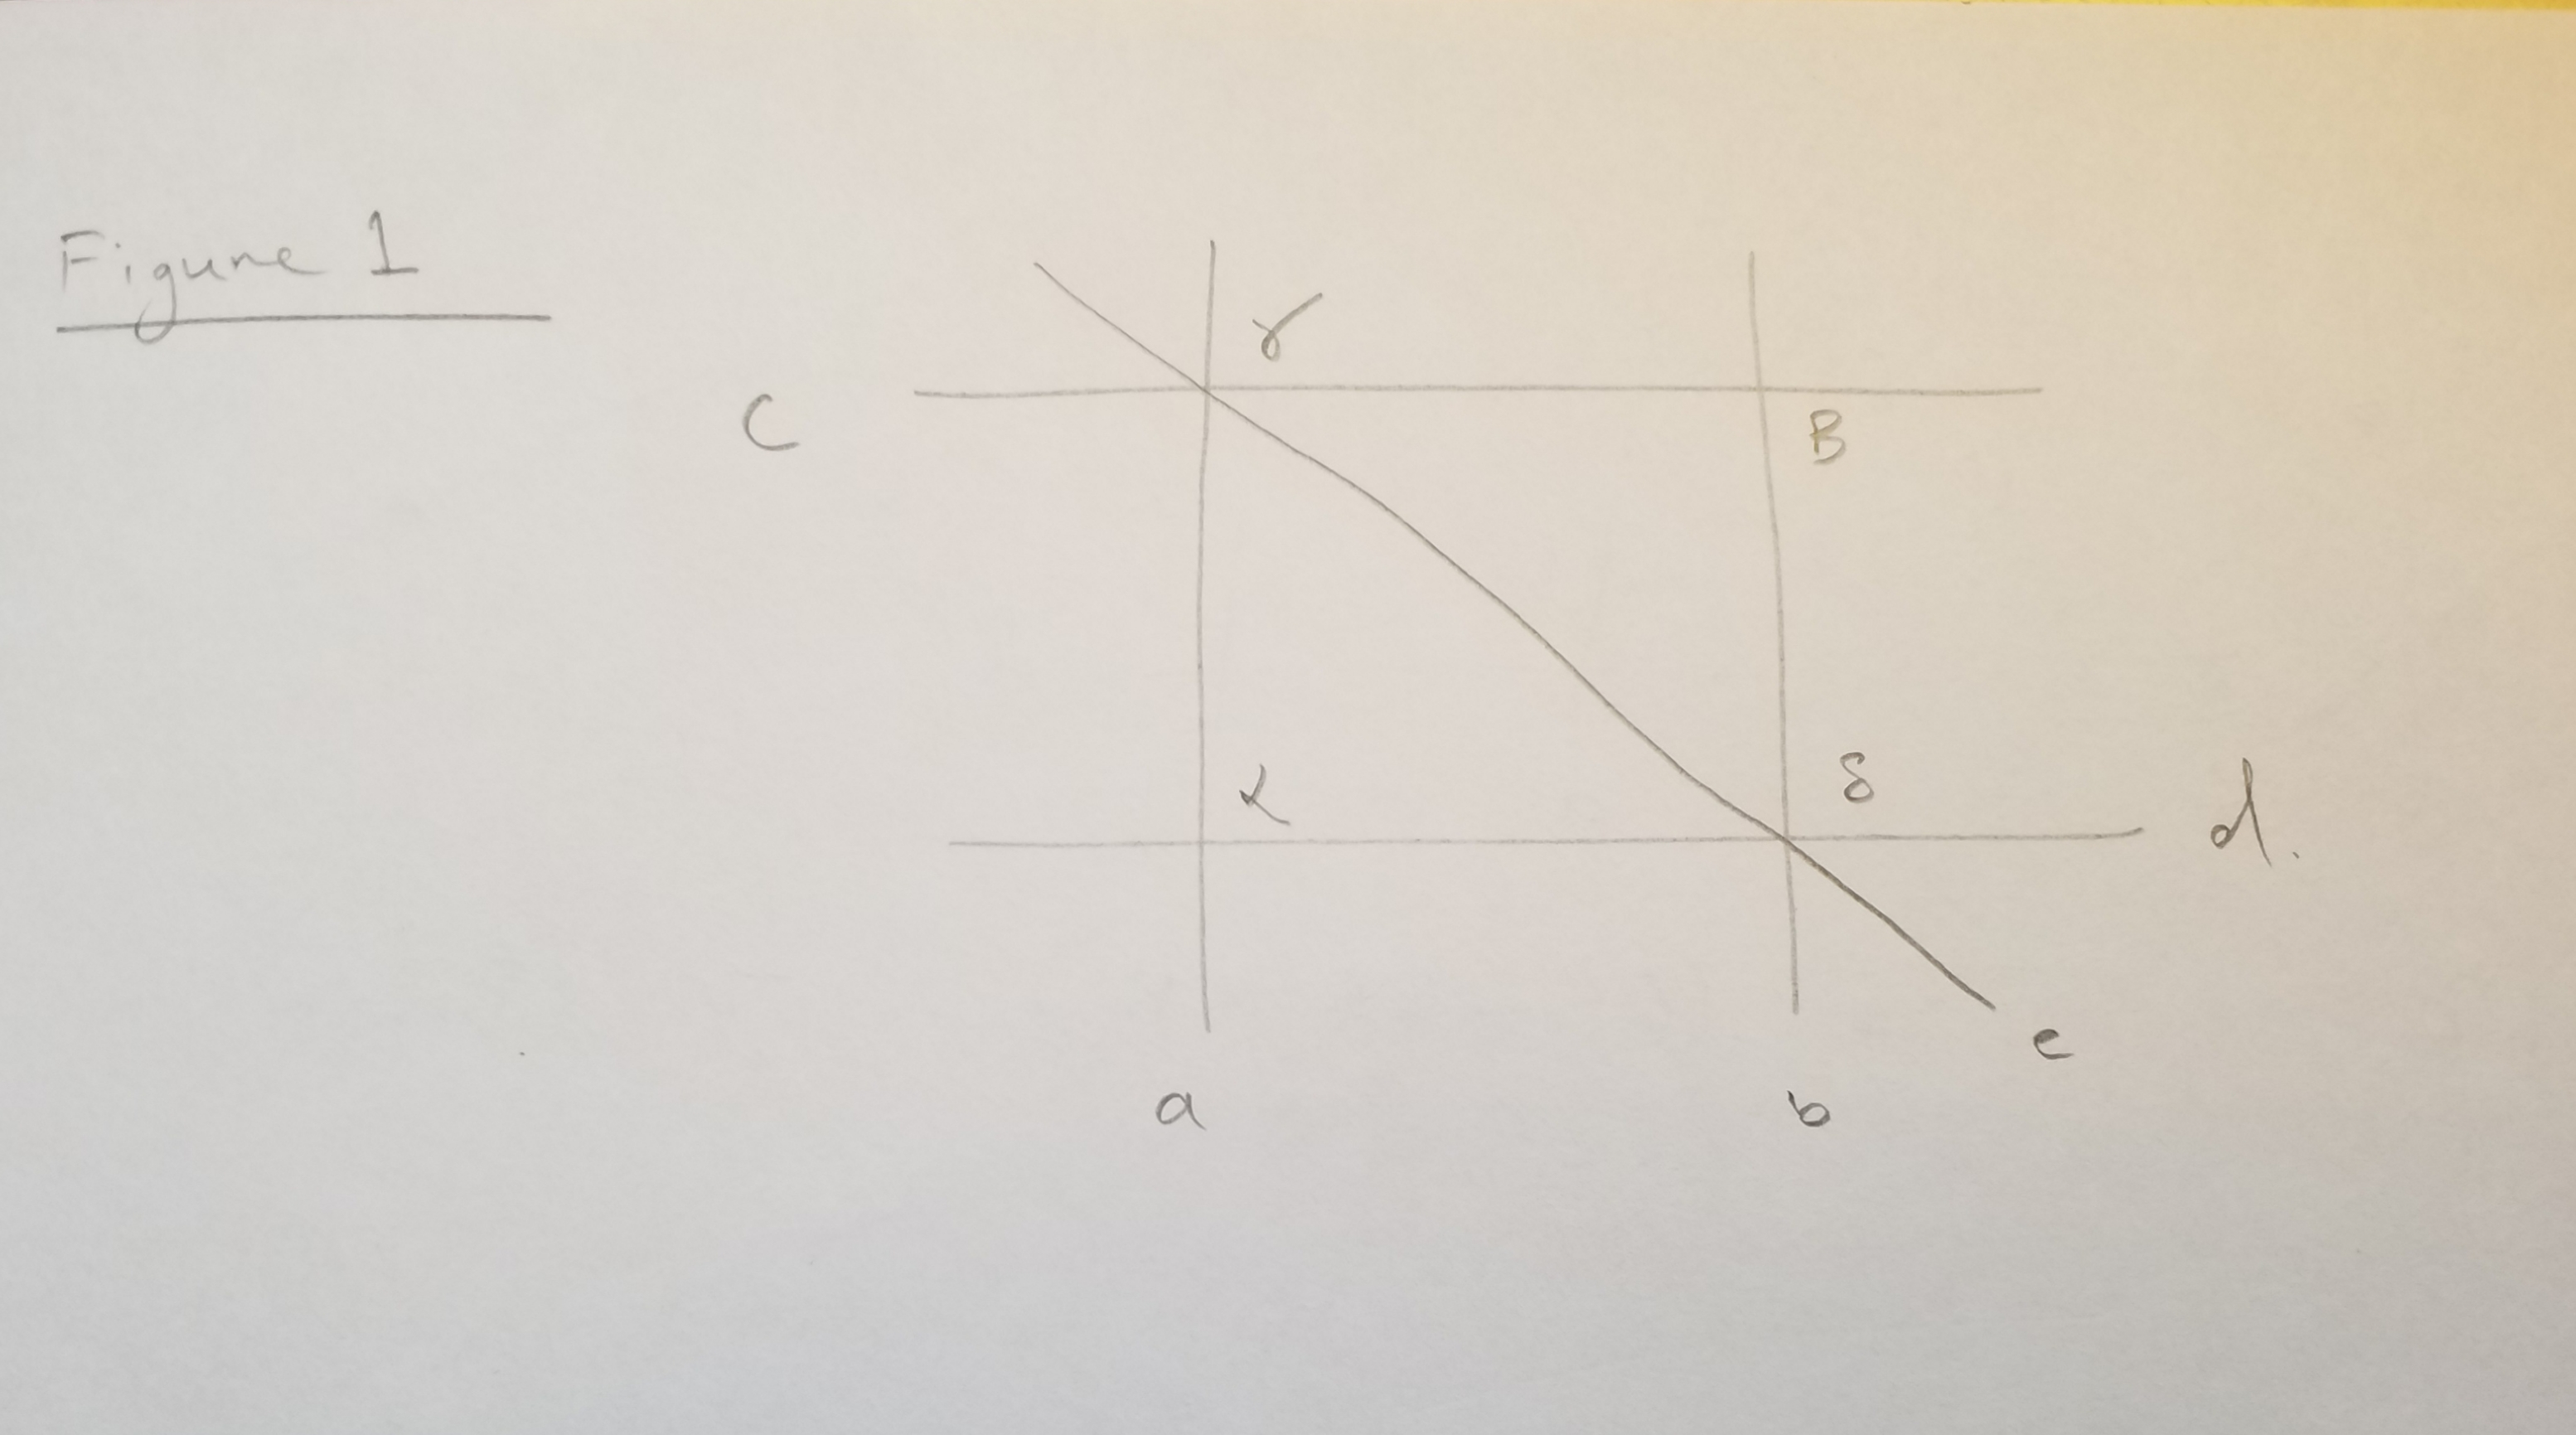
\includegraphics[scale=0.10,angle=0]{29072020 pics/fig 1.jpg}  
    \caption{Hyperplane arrangement in $\mathbb{R}^2$.}
    \label{fig 1}
\end{figure}

It is important to distinguish between unbounded and bounded regions. Note hyperplane arrangements are denoted by $\mathcal{A}$.

\begin{definition}
A region is a connected component of,
        $\mathbb{R}^n \setminus \cup_{H \in \mathcal{A}} H$. The set of regions is $\mathcal{R}(\mathcal{A})$ and the number or regions is $r(\mathcal{A})=\#\mathcal{R}(\mathcal{A})$. The term $b(\mathcal{A})$ is the number of bounded regions in the standard sense. 

\end{definition}

 \begin{definition}\label{Intposet}
 Let $\mathcal{A}$ be an arrangement in $\mathbb{R}^n$, and let $L(\mathcal{A})$ be the set of all nonempty intersections of hyperplanes in $\mathcal{A}$, including $\mathbb{R}^n$. Define $x \le y $ in $L(\mathcal{A})$ if $x \subseteq y$. That is $L(\mathcal{A})$ is partially ordered by reverse inclusion. Call $L(\mathcal{A})$ the intersection poset of $\mathcal{A}$.
 \end{definition}
 
 These intersections are often called flats. We assign a value, $\mu(x)$, to each flat in $L(\mathcal{A})$.

\begin{definition}\label{mob} Let $P$ be a locally finite poset. Define the Möbius function to be $\mu : Int(P) \rightarrow \mathbb{Z}$ by 

\begin{align*}
    \mu (x,x) &=1, \quad \forall x \in P\\
    \sum _{x \le z\le y} \mu(x,z)&=0, \quad \forall x<y \in P
\end{align*}

and $\mu(x)=\mu(\hat{0},x)$.

\end{definition}

\begin{remark}
  Each hyperplane has mobius value $-1$.
\end{remark}

\begin{example}{Example of intersection poset with mobius values and with non-generic line in $\mathbb{R}^2$}
\begin{figure}[H]
    \centering
 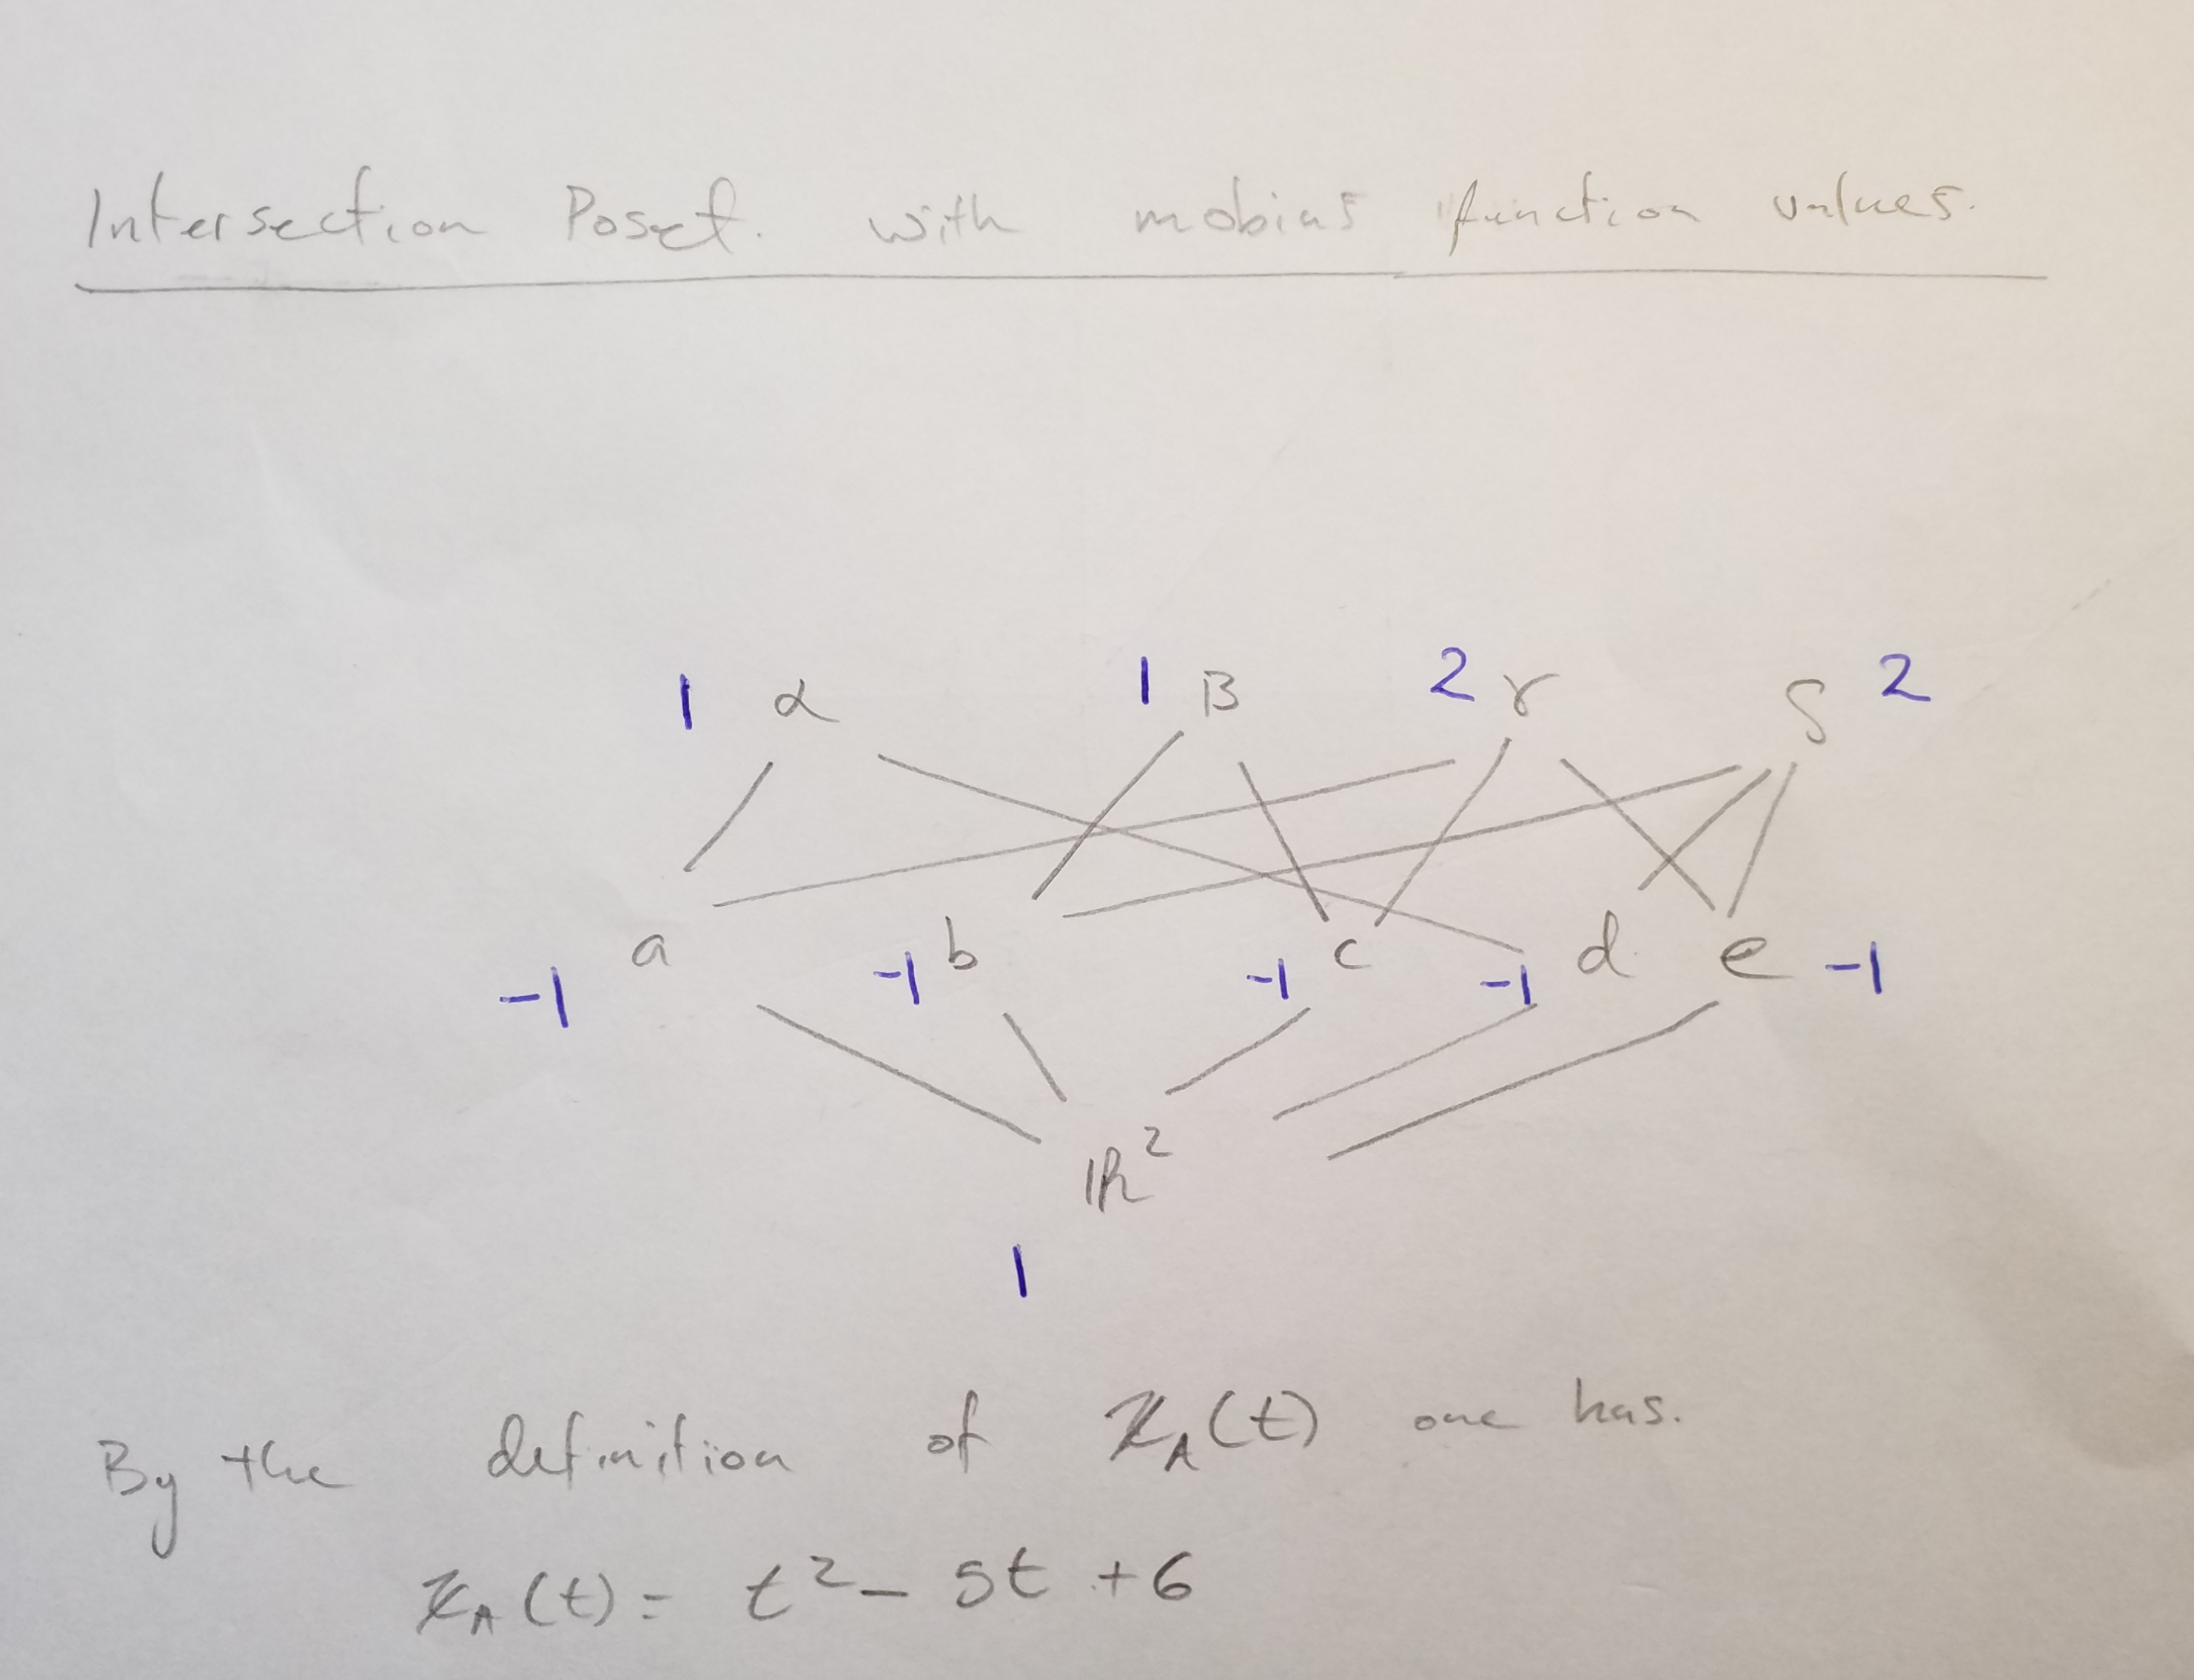
\includegraphics[scale=0.10,angle=0]{29072020 pics/poset.jpg}  
    \caption{Intersection poset of Figure 1 with Möbius values.}
    \label{poset1}
\end{figure}
\end{example}

 \begin{remark}
    In $\mathbb{R}^2$ lines are either parallel or intersect at a point, points either live outside of line or embedded in a line. In $\mathbb{R}^3$ planes either intersect giving a line or are parallel. For lines and planes, either lines are embedded, intersect at a point or are disjoint. By generic we mean, we exclude the special cases of what we mentioned above. For a total space of dimension $n$, with $k$ hyperplanes in general position, when all hyperplanes intersect they give a "subspace/set" of $codim = k$. Non-generic behaviour effects the mobius value. The flat $\gamma$ in Figure \ref{poset1} is not generic as we get a point and expect the empty set. If hyperplanes are in generic position, this gives a total of $2^k$ regions.
 \end{remark}
 

\begin{definition}
The characteristic polynomial $\chi_{{\mathcal{A}}} (t)$ of $\mathcal{A}$ is,

$$\chi_{\mathcal{A}} (t) = \sum_{x \in L(\mathcal{A})}  \mu (x) t ^{\text{dim} (x)} $$
\end{definition}

\begin{example}

This is an example of a central arrangement with which is non-generic in $\mathbb{R}^3$.

\begin{figure}[H]
    \centering
    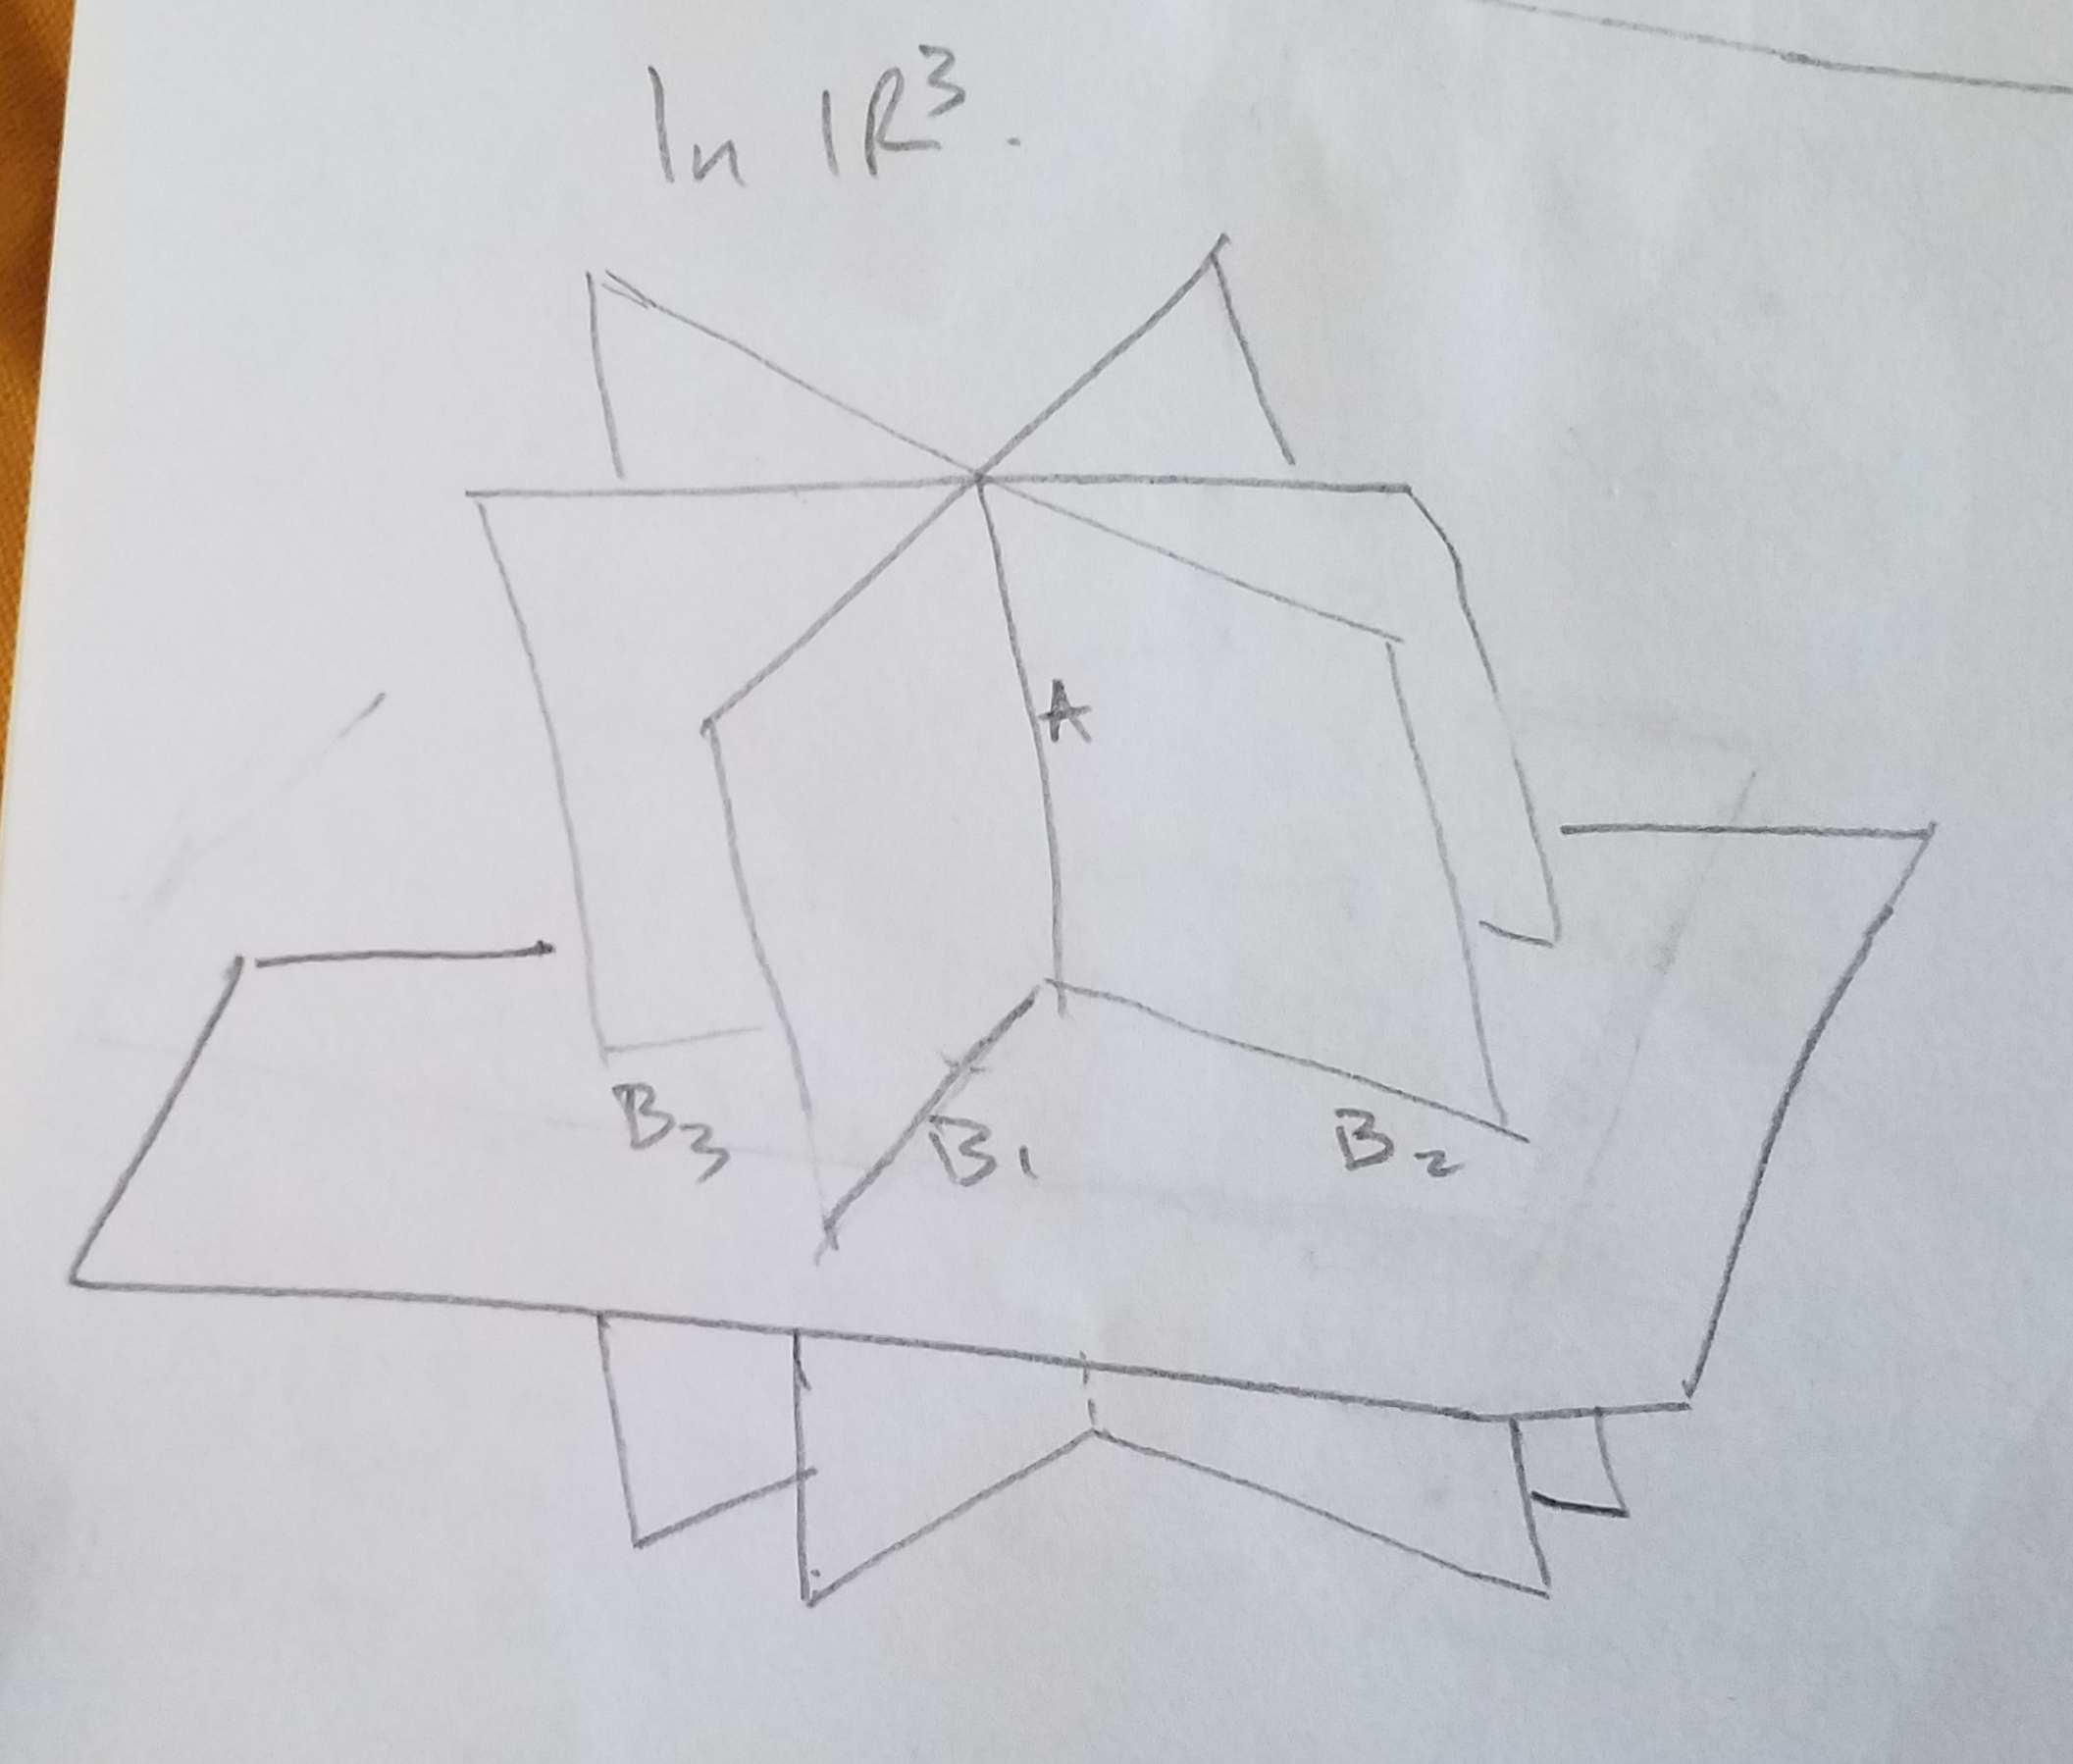
\includegraphics[width=.5\textwidth]{29072020 pics/arrg.jpg}
    \caption{Arrangement in $\mathbb{R}^3$}
    \label{Arranmgnet in R^3}
\end{figure}

Which has the following poset with associated mobius values. 

\begin{figure}[H]
    \centering
    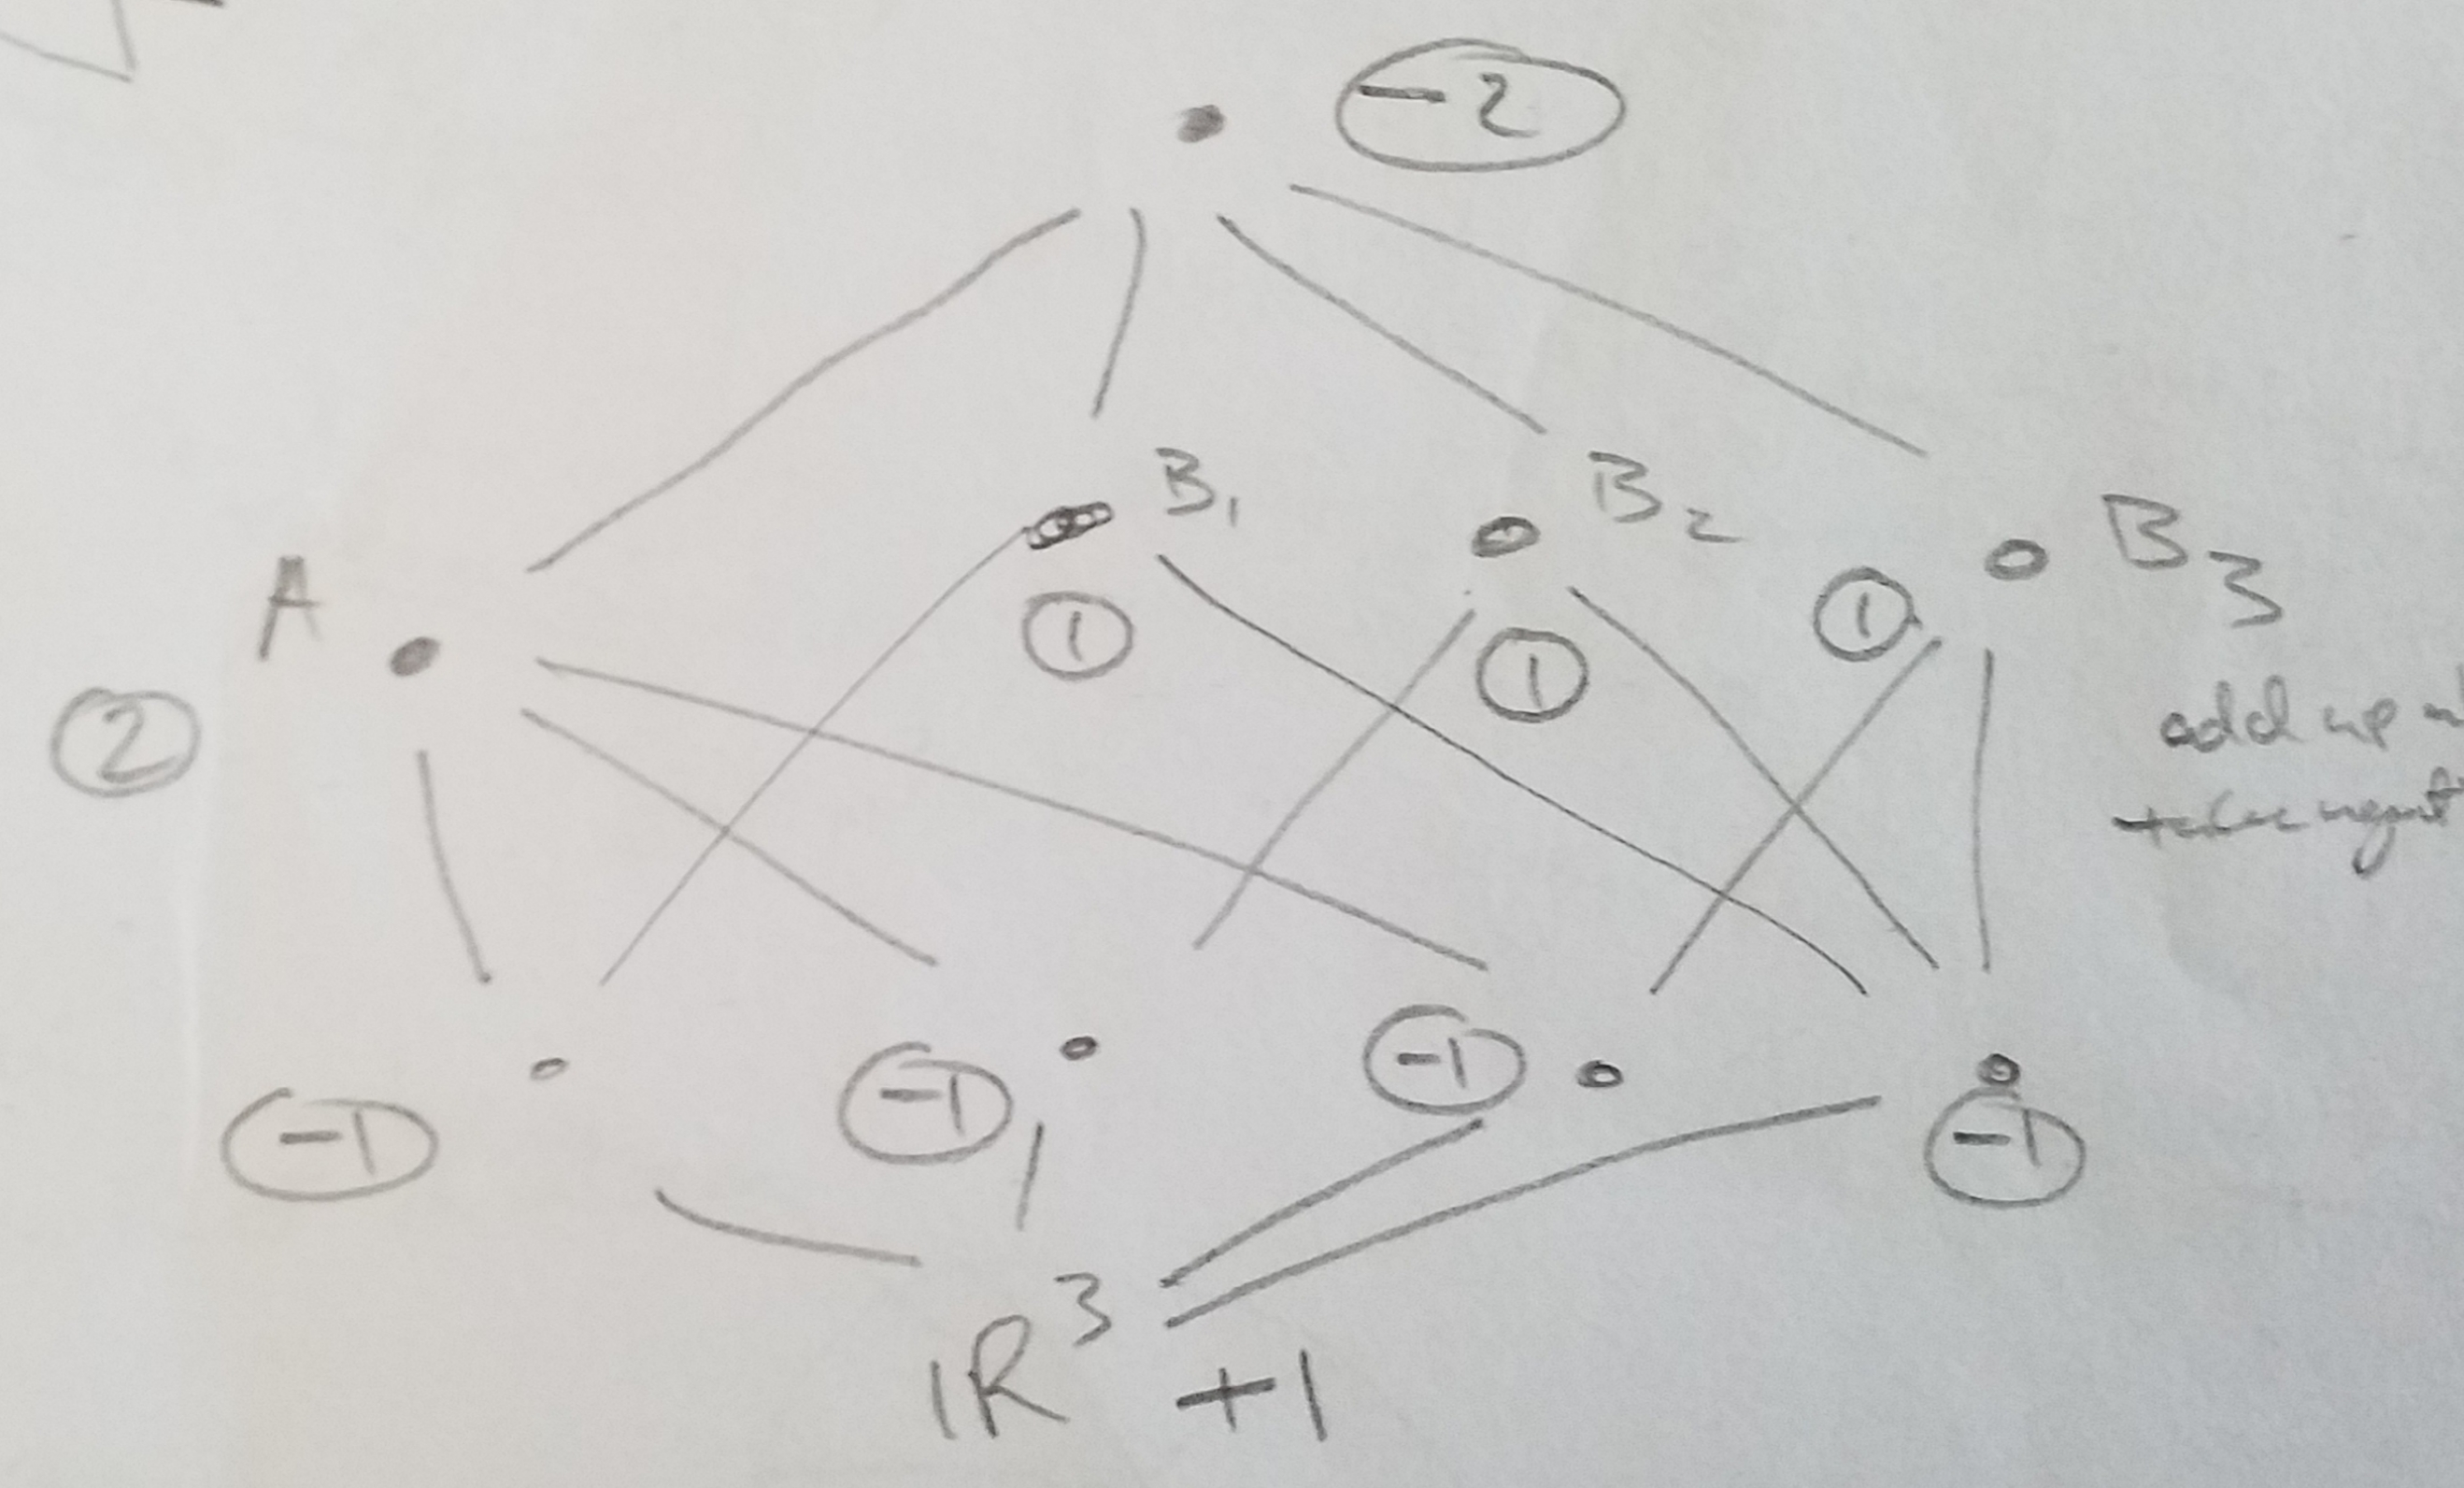
\includegraphics[width=.5\textwidth]{29072020 pics/posetarrg.jpg}
    \caption{Poset with mobius values of Figure \ref{Arranmgnet in R^3}} 
    \label{fig:my_label}
\end{figure}



The characteristic polynomial measures the complement of the arrangement. Consider the whole space ($t^3$),then remove the hyperplanes ($-4t^2$), in doing so we removed the three lines $B_1,B_2$ and $B_3$, and the line $A$ is removed a further $2$ times, so we correct by adding ($+5t$). In adding the lines back we have two additional orgins points, so we correct with $-2$. The characteristic polynomial is hence, $\chi(\mathcal{A})=t^3-4t^2+5t-2$.
\end{example}




The rank$(\mathcal{A})$ is the dimension of the space spanned by the normal's of hyperplanes in $\mathcal{A}$, when this agrees with $dim(\mathcal{A})=dim(\mathbb{R}^n$, $\mathcal{A}$ is called essential. One obtains this through the process of essentialization.  

\begin{theorem}\label{Zas}[Zaslavsky's theorem, \cite{stanley2004introduction}, Thm 2.5, p.19] Let $\mathcal{A}$ be an arrangement in $\mathbb{R}^n$. Then $r(\mathcal{A})=(-1)^n \chi_{\mathcal{A}} (-1)$ and $b(\mathcal{A})=(-1)^{\text{rank}(\mathcal{A}) }  \chi_{\mathcal{A}} (1)$. 

\end{theorem}

In order to determine $b(\mathcal{A})$ in the case of $H(S,k)$, we need to know $\chi_{{\mathcal{A}}} (t)$. The issue here, is to determine $L(\mathcal{A})$ and $\mu(x)$ for large $n$, (\cite{Etu} gives a program for this however it grows exponentially with $n$). 

\section{Applying Zaslavsky's Theorem to the Resonance Arrangement in $\mathbb{R}^2$ and $\mathbb{R}^3$}

Consider the following arrangement, where all hyperplanes are positioned at the origin. The number of regions for each $n$, belong to the following OEIS reference: A034997.

\begin{example}
Take the $\mathbb{R}^2$ case with $x=0,y=0, x+y=0$. 

\begin{figure}[H]
    \centering
 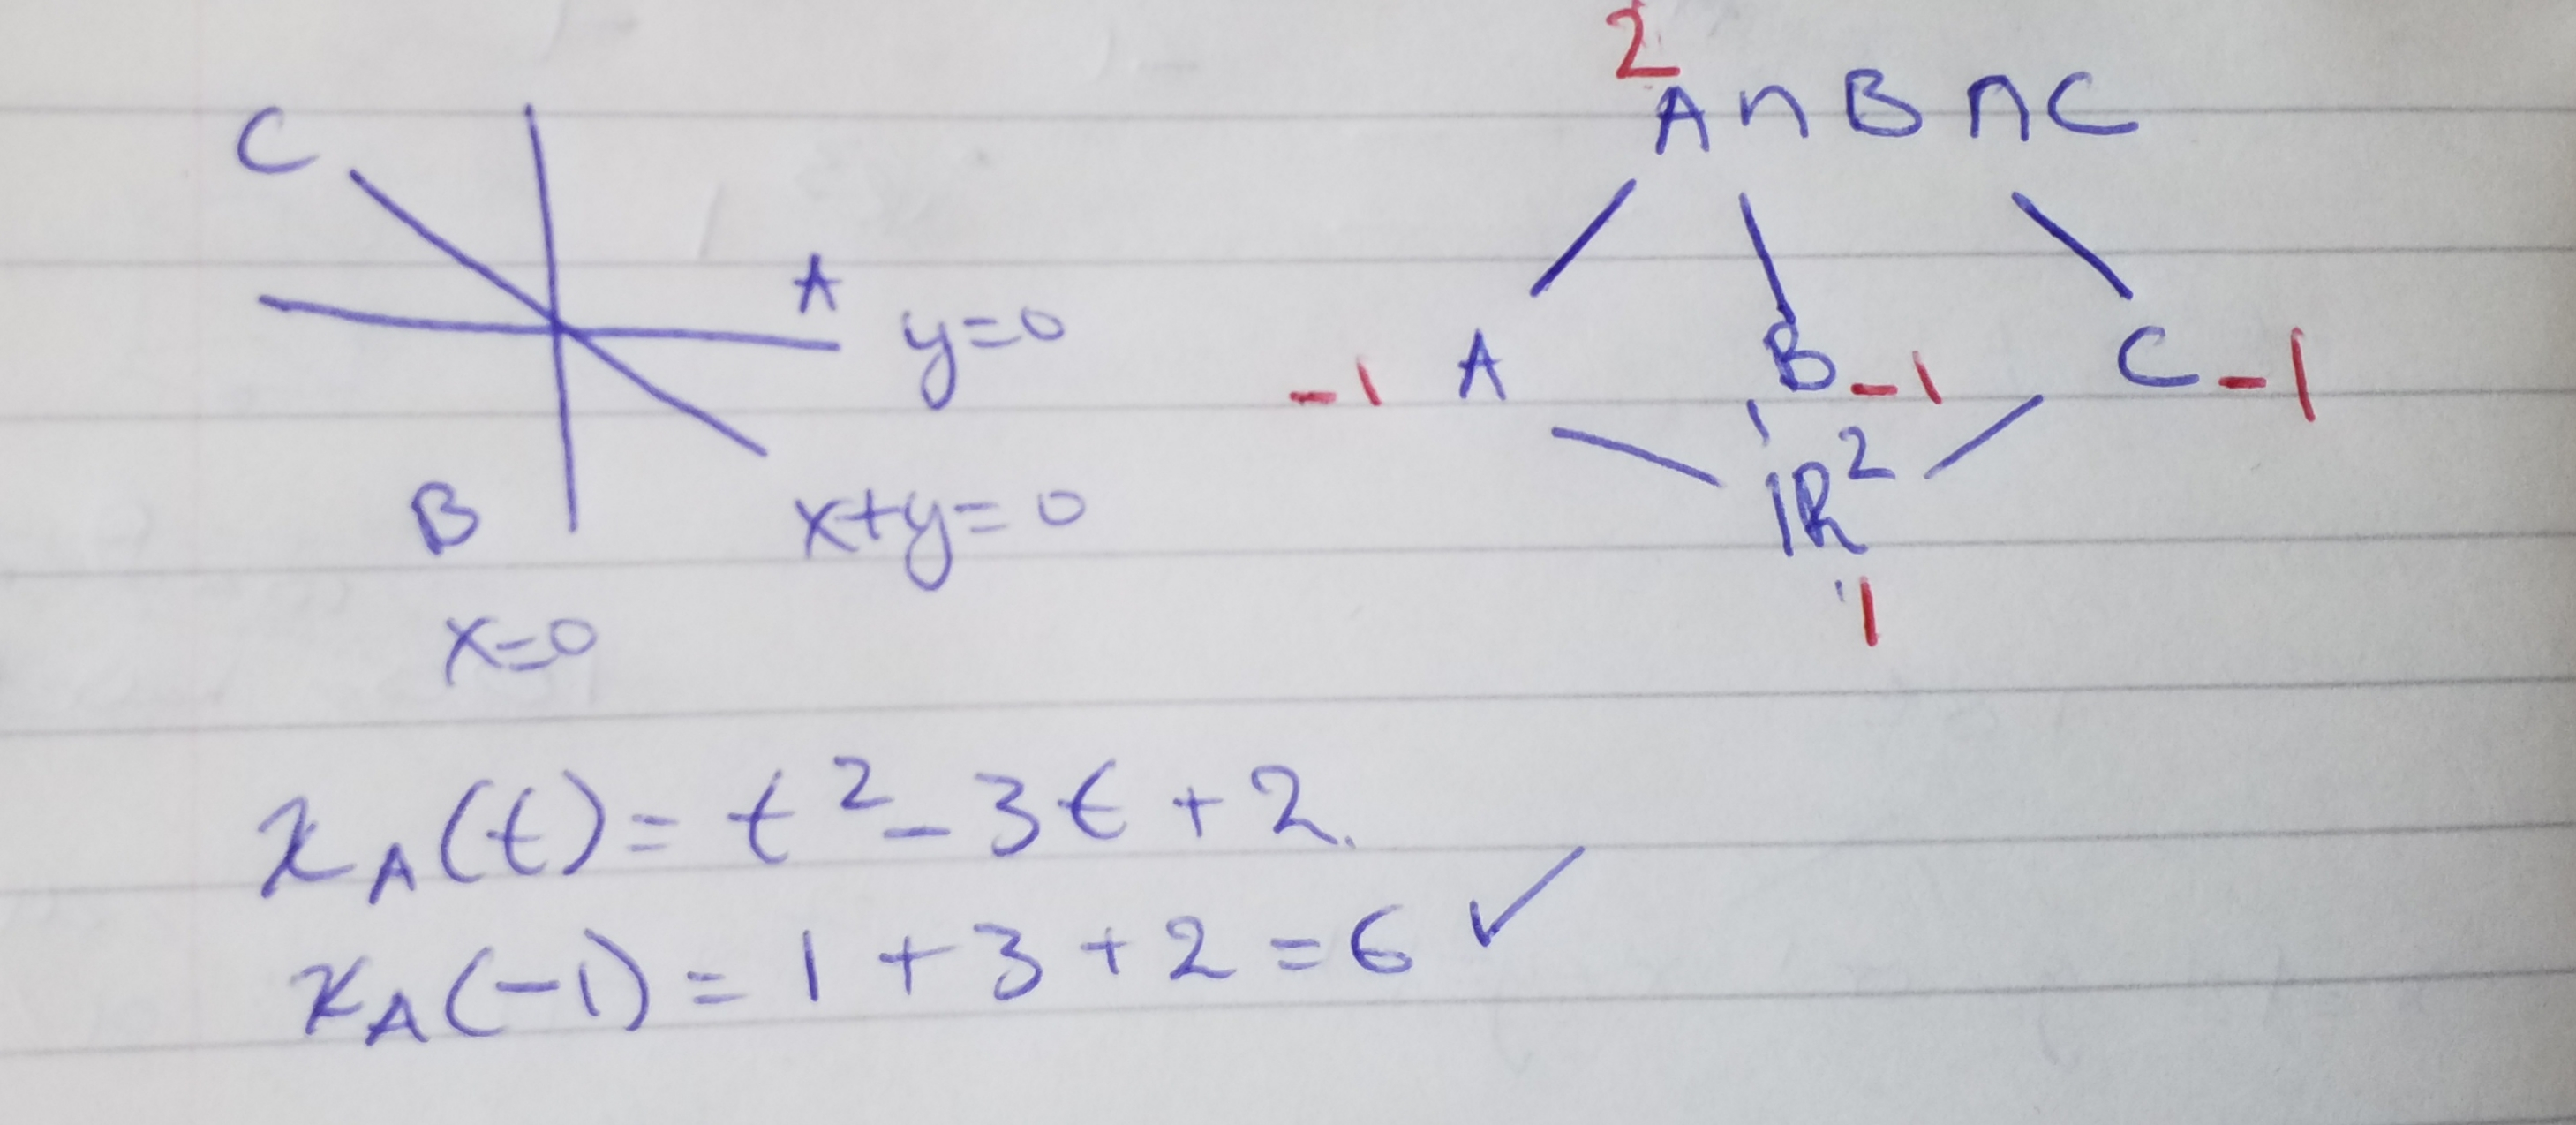
\includegraphics[scale=0.10,angle=0]{29072020 pics/resonance R2.jpg}  
    \caption{Number of region resonance arrangement $\mathbb{R}^2$}
    \label{res}
\end{figure}
\end{example}


\begin{example}
Apply Zaslavsky's theorem to the $\mathbb{R}^3$ resonance arrangement case.

\begin{figure}[H]
    \centering
 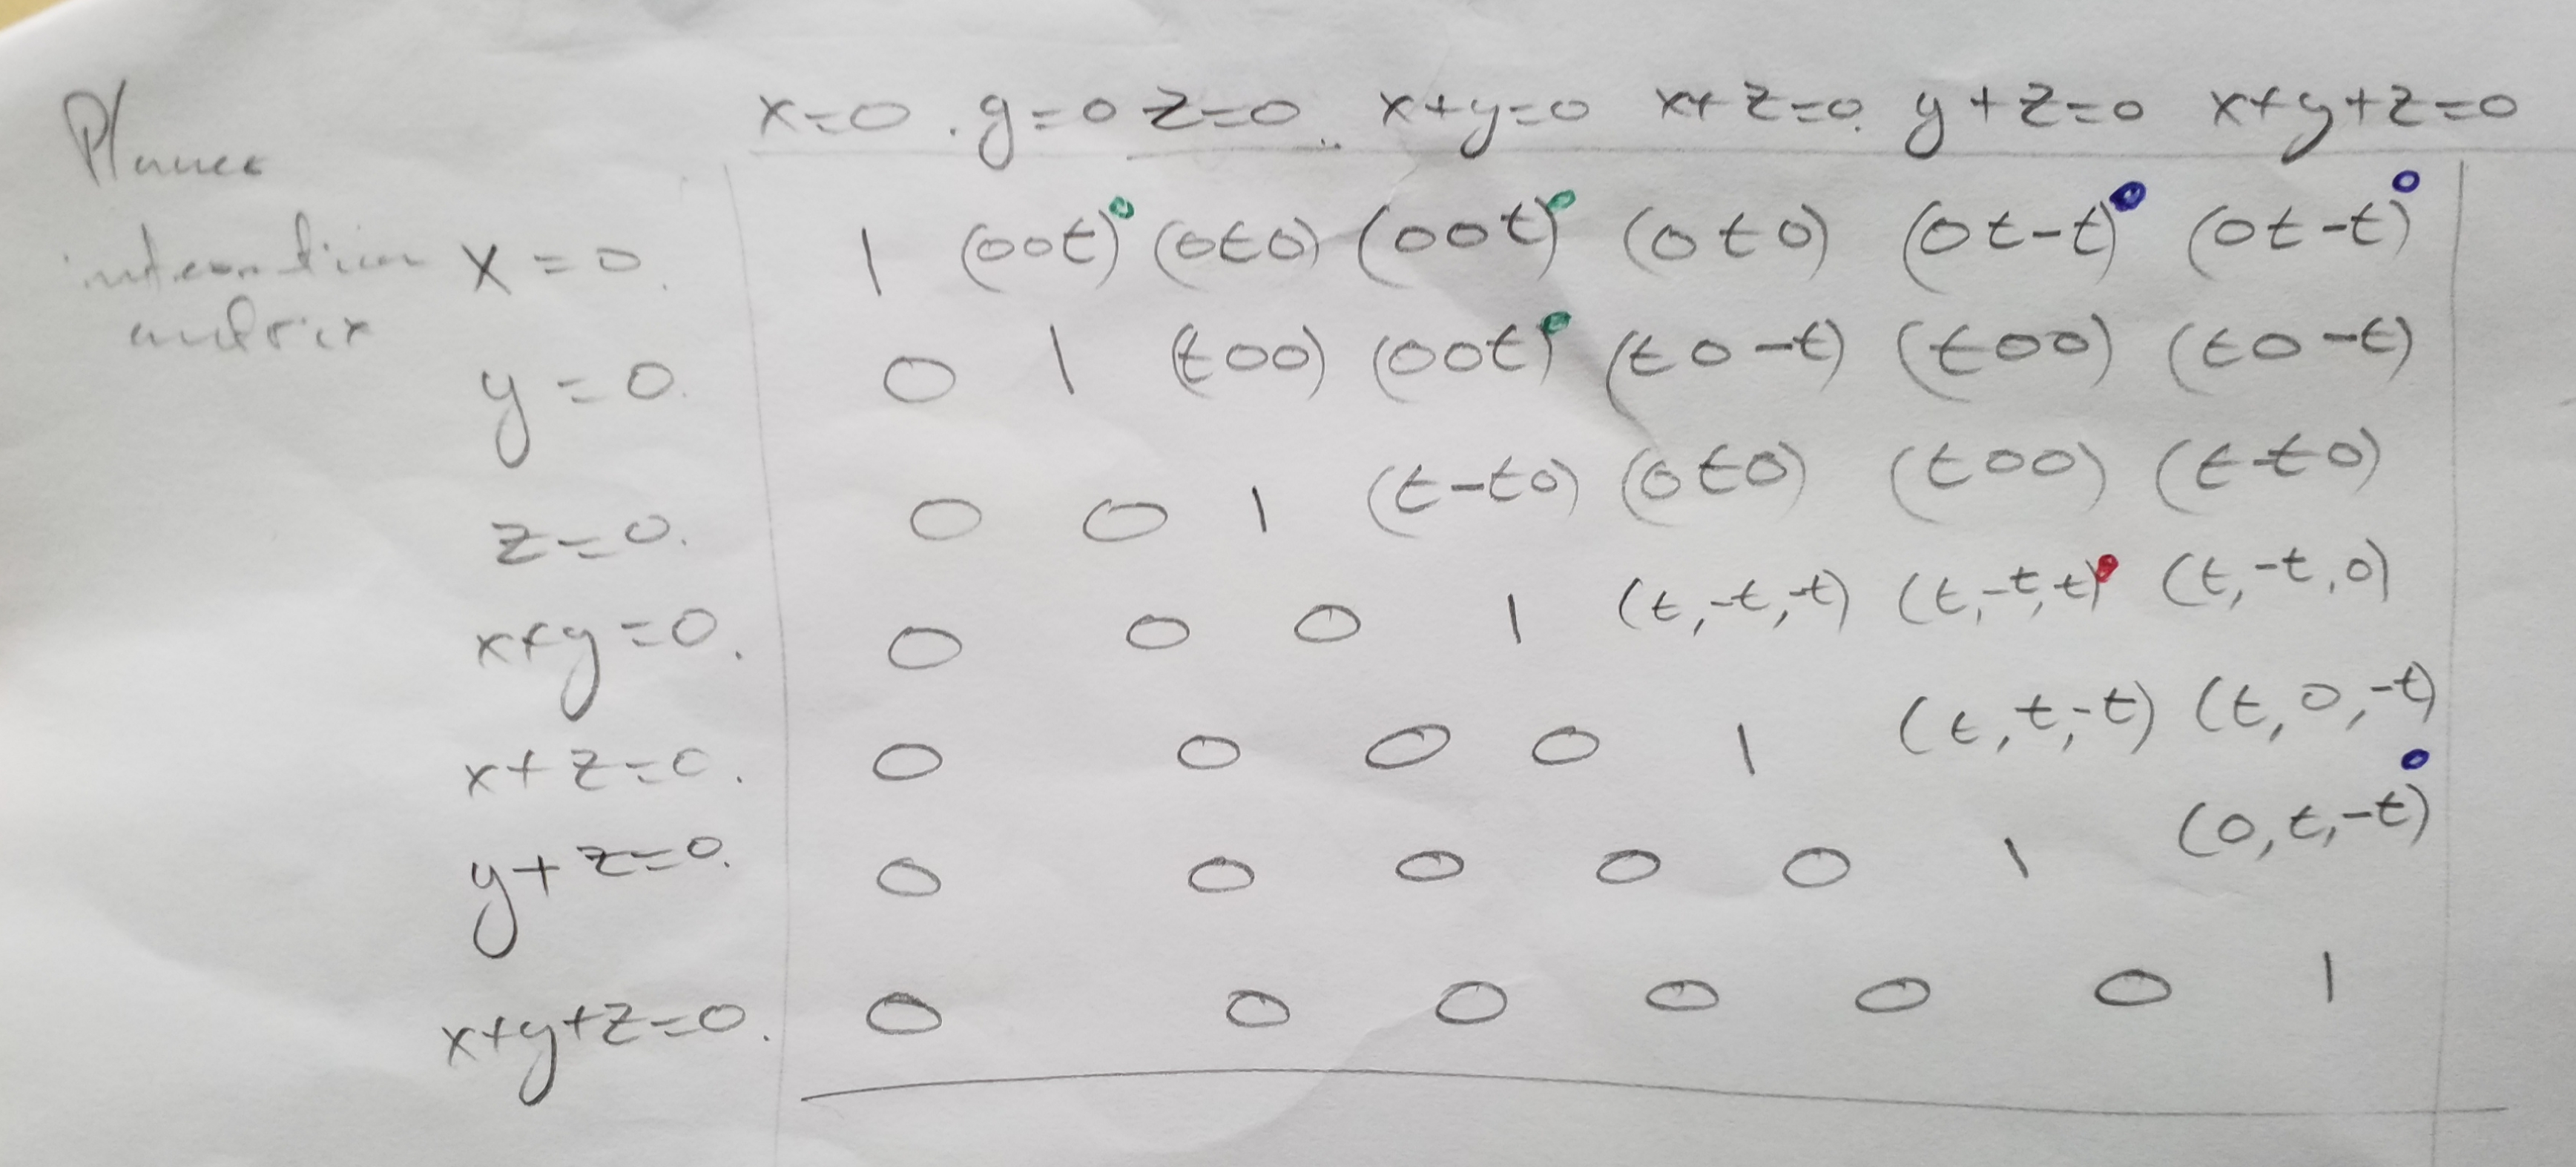
\includegraphics[scale=0.10,angle=0]{29072020 pics/resplaneeintersect.jpg}  
    \caption{Plane intersection matrix }
    \label{res}
\end{figure}



All planes intersect at the origin and recall each plane has mobius value $-1$. Each line that appears once in Figure \ref{res} is from two separate planes and so has mobius value $1$. If it appears three times it is from three planes and of mobius value $2$. We summaries this data as,

\begin{center}
\begin{tabular}{ |c|c|c|c|c|c|c|c|c|c|c| } 
 \hline
Line &(0,0,t)& (0,t,0)& (t,0,0) & (t,-t,0) & (0,t,-t) & (t,0,-t) & (t,-t,t) & (t,t,-t) & (t,-t,-t) \\ 
\hline
$\mu$ &2& 2& 2& 2& 2& 2 & 1 & 1 &1\\
\hline

 \hline
\end{tabular}
  \caption{} \label{tab:sometab}
\end{center}

There are seven planes in total and the sum of the mobius values for lines is $15$. Therefore by definition \ref{mob} we have, 

$$ 1 - 7 +15 + \mu(origin)=0$$

and so $\mu(origin)=9$. Applying Zaslavsky's theorem, we have $r(\mathcal{A})= 1+7+15+9=32$ and $b(\mathcal{A})=0$. 

\end{example}



 \section{Applying Zaslavsky theorem to $H(S,k)$ in the affine case of $\mathbb{R}^2$ and $\mathbb{R}^3$}

 In order to apply the classical Zavalaskys theorem (for a finite arrangement) we need to make a choice of hyperplanes from the family $H(S,k)$ (equation \ref{HSK}). In the $\mathbb{R}^2$ the choice given in Figure \ref{fig 1} gives the correct number of bounded regions if one chooses only $x+y=1$, and not for example if we choose the lines $x+y=0, x+y=1, x+y=2$.
 
 \begin{figure}[H]
    \centering
 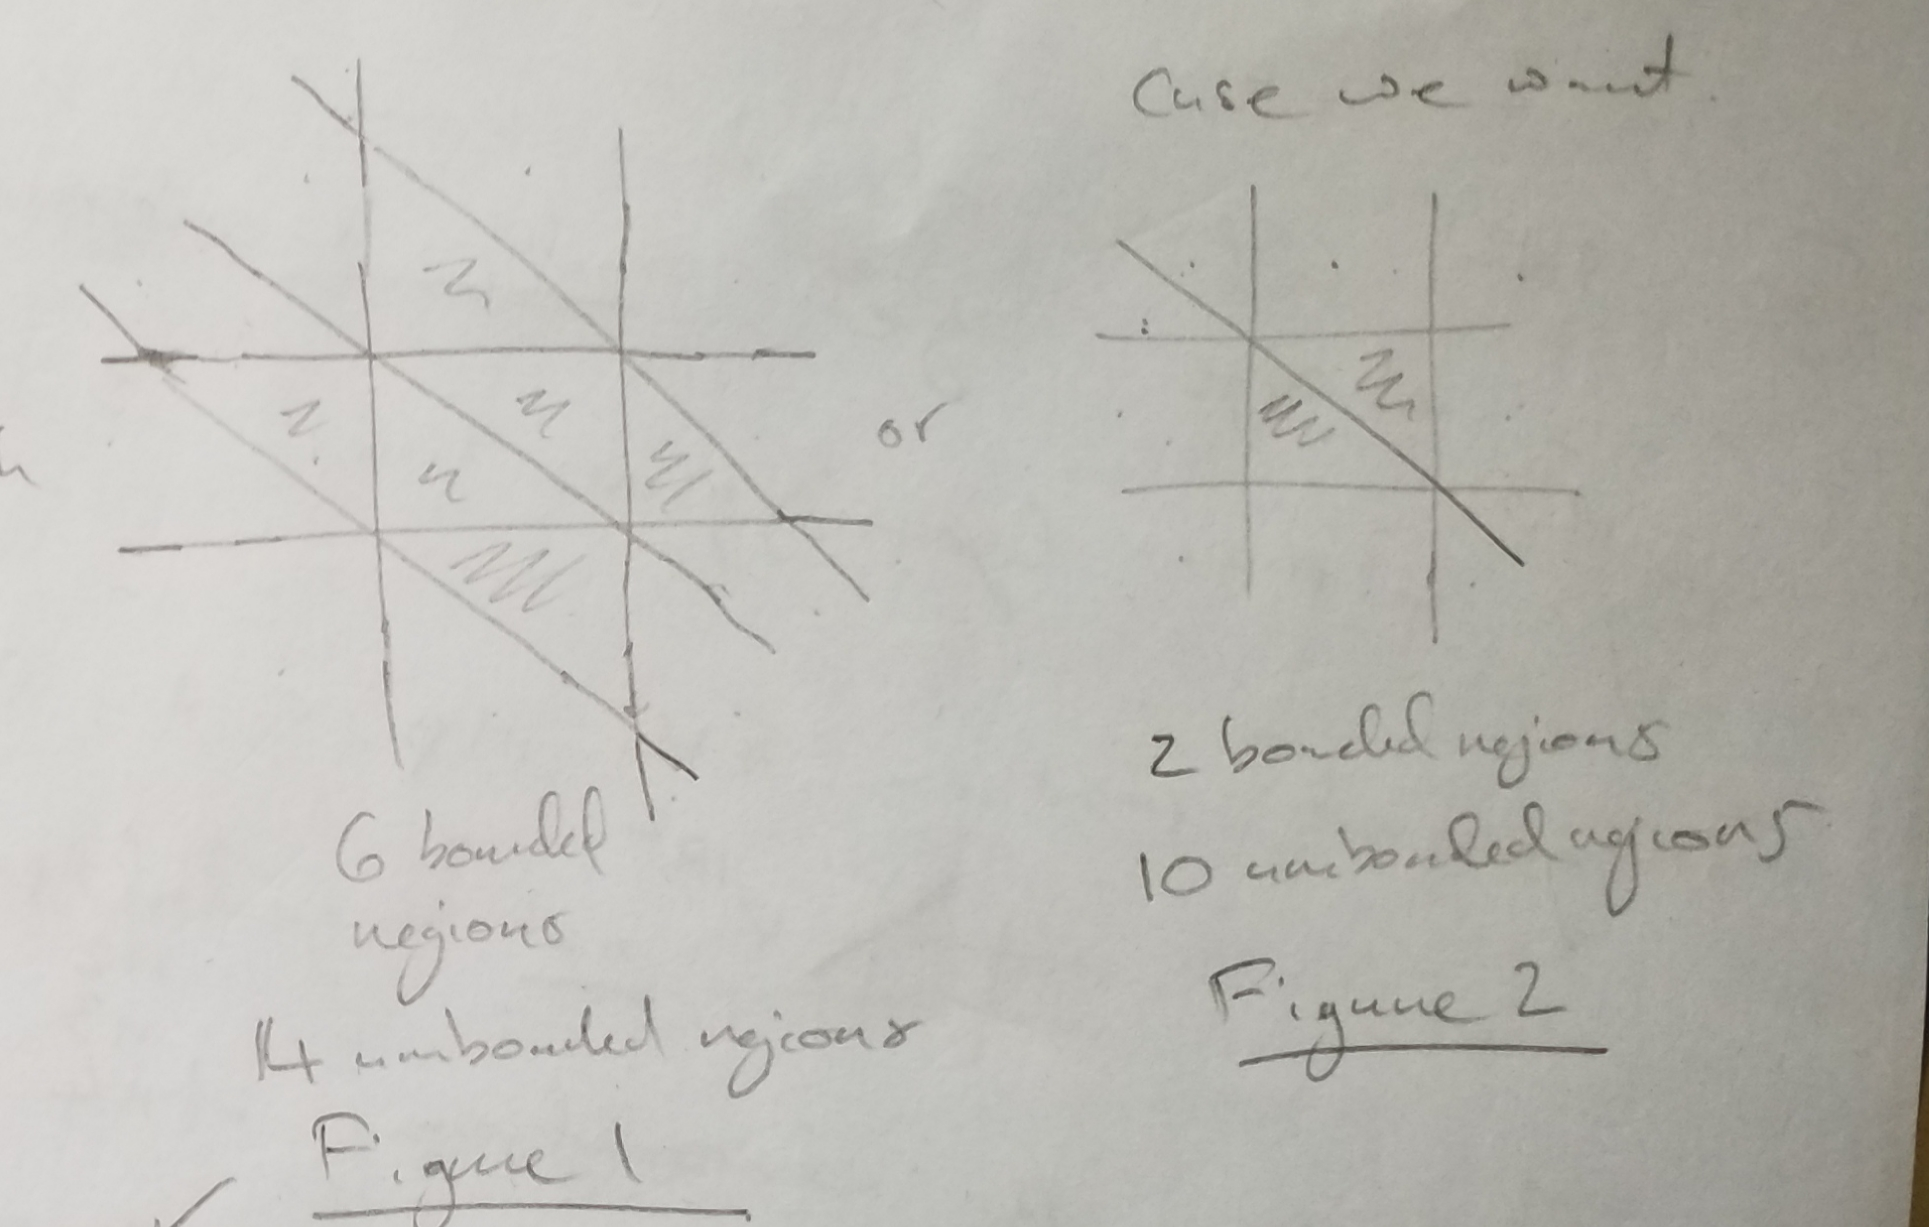
\includegraphics[scale=0.15,angle=0]{29072020 pics/n=4 choice lines.jpg}  
    \caption{Choosing the correct lines from $H(S,k)$}
    \label{fig 6}
\end{figure}
 
 Therefore we are choosing to only include those lines that intersect the interior of the square and not count those that meet the interior and boundary (left diagram of Figure \ref{fig 6}). Generalising to $\mathbb{R}^3$ case, we have the following problem. 
 To apply Zaslavsky's theorem to the following arrangement $\mathcal{A}$ given by the equations of (\ref{HSK}) and determine $b(\mathcal{A})$. We have determined (using geoalgebra and inspection) the number of bounded regions inside the cube to be $10$. Is $b(\mathcal{A}) =10$ if one constructs $L(\mathcal{A})$ and applys Zaslavsky's theorem. If we find a number greater than $10$ then the method of taking the interior planes does not work and we must find a different approach. The suggested next step is to consider toric hyperplane arrangements. 
 
\begin{example}
Consider the arrangement $\mathcal{A}$ $x,y,z= 0,1$, $x+y=1$, $y+z=1$, $x+z=1$, $x+y+z=1$, $x+y+z=2$ in $\mathbb{R}^3$. We aim to determine the intersection poset and the Möbius values of each element, then determine the characteristic polynomial, and then $b(\mathcal{A})$. First we determine the lines of intersection of all pairs of planes.

\begin{figure}[H]
    \centering
 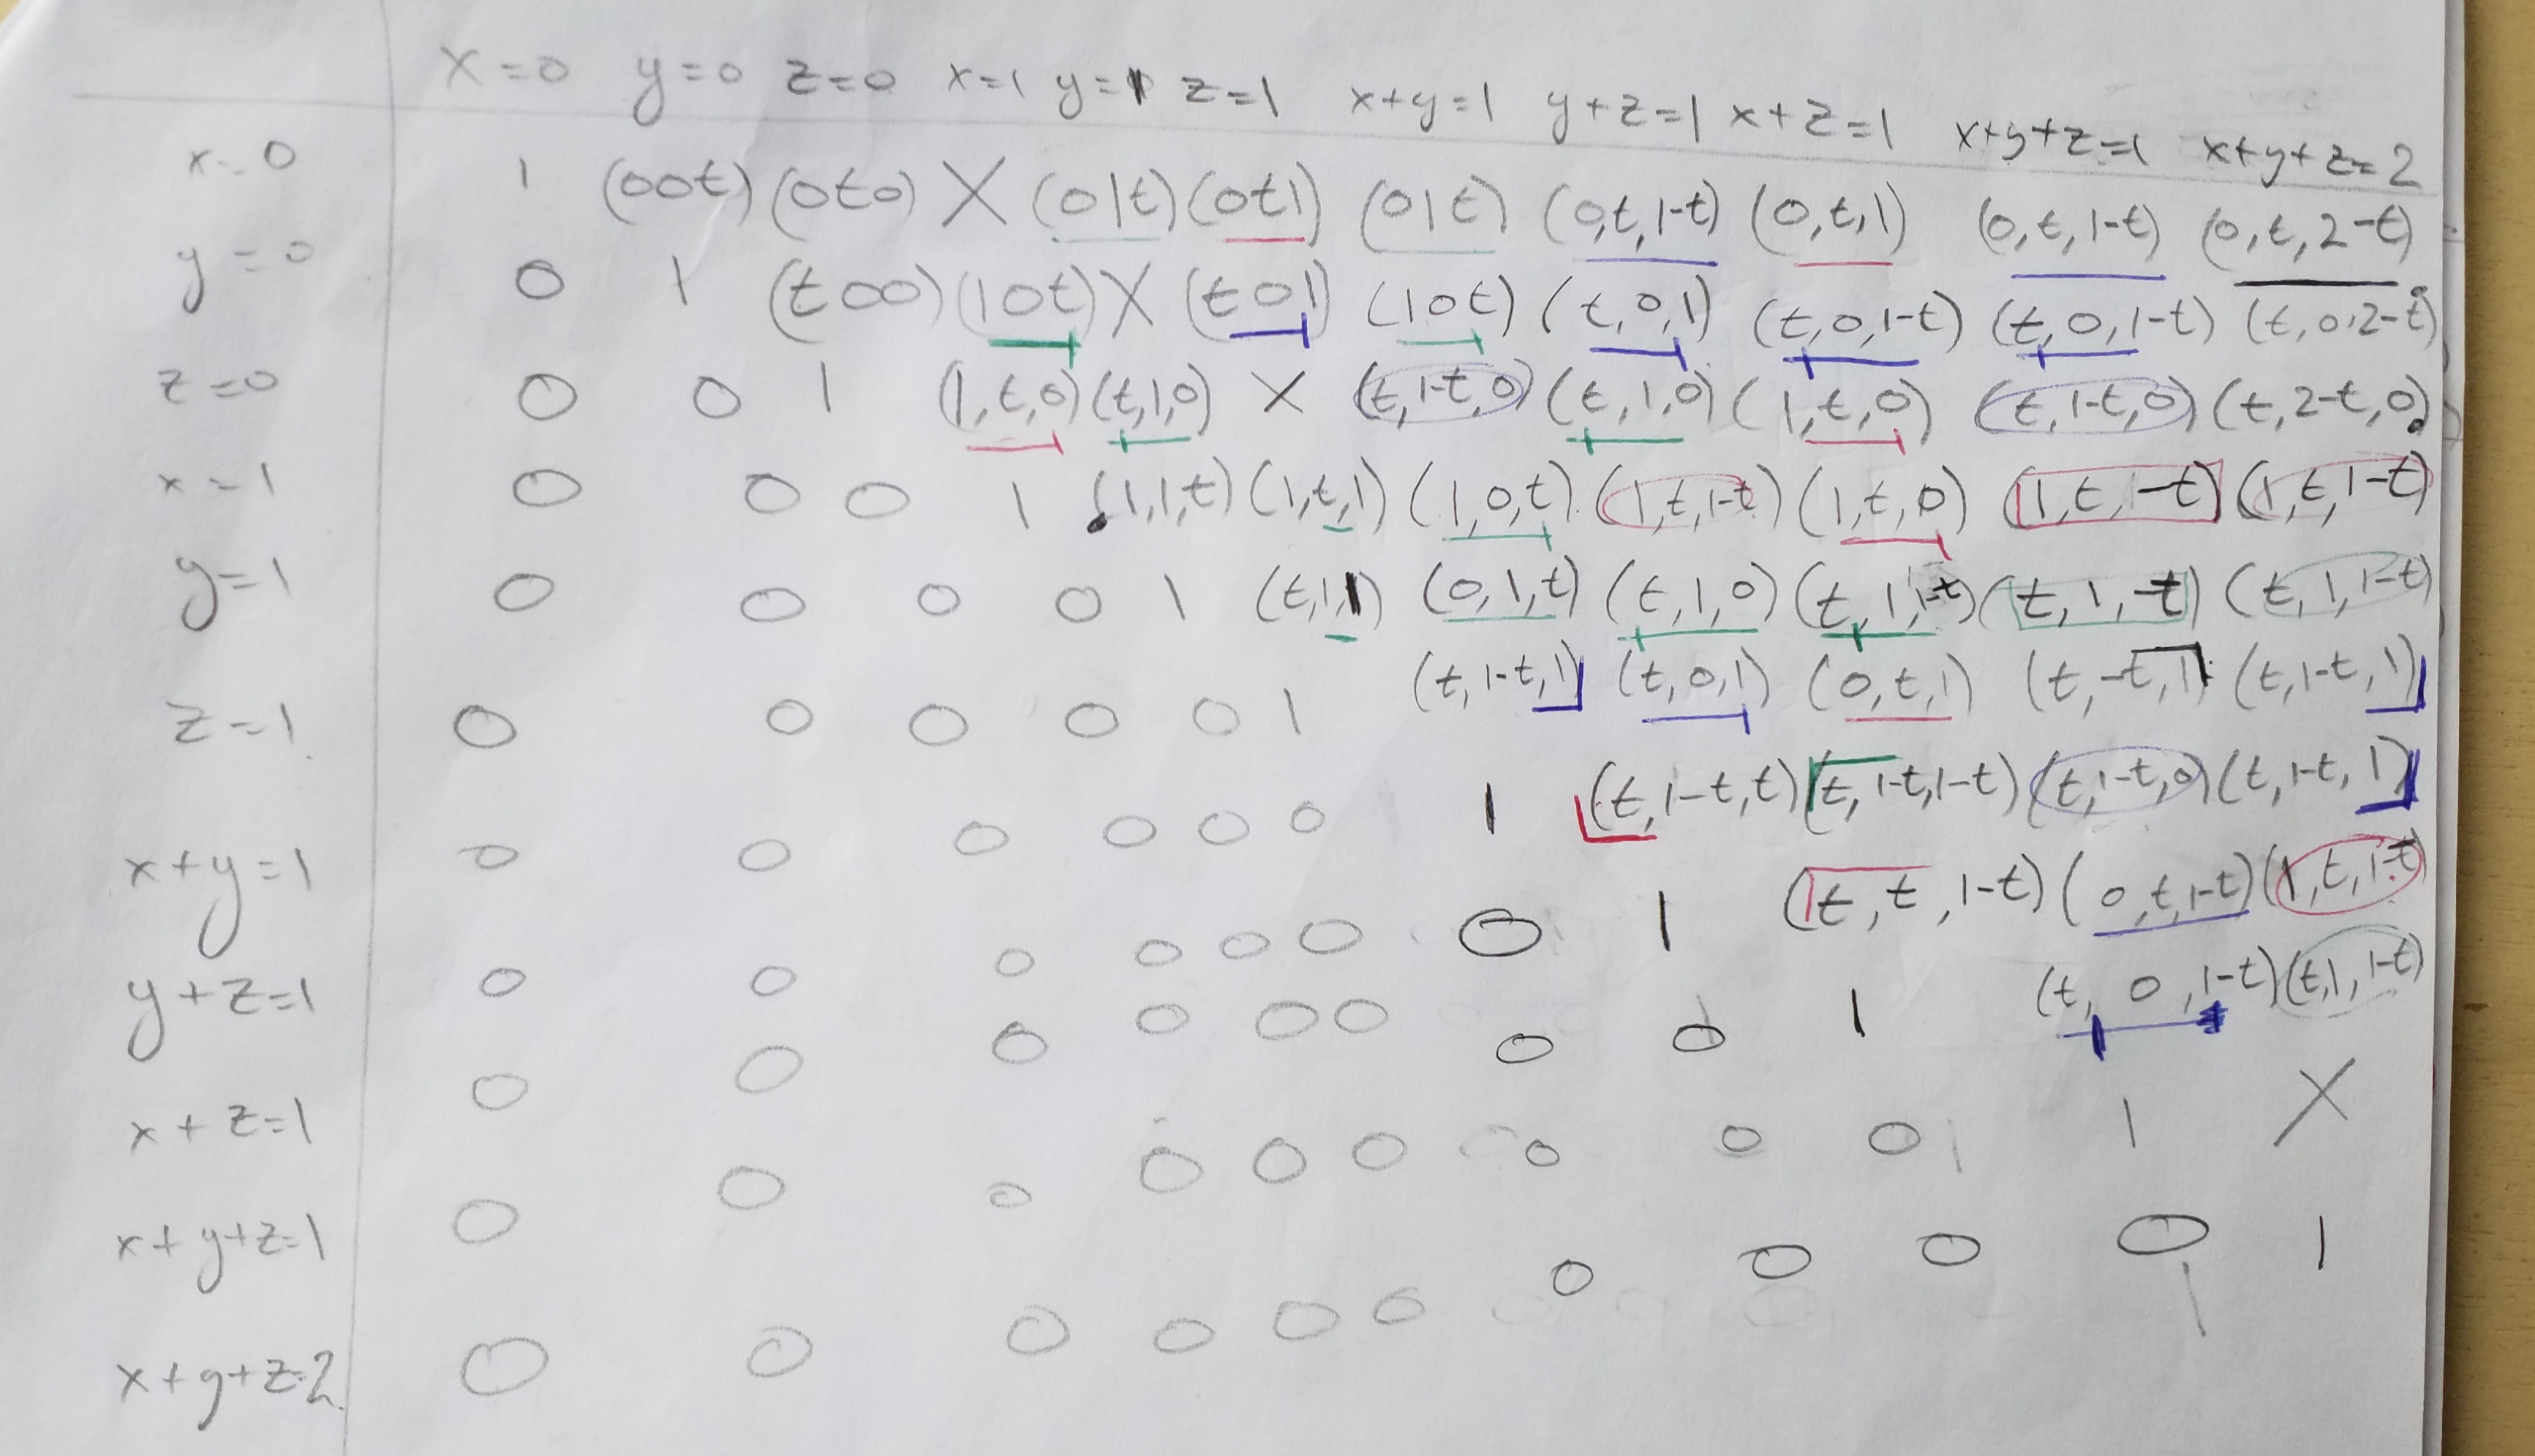
\includegraphics[scale=0.10,angle=0]{29072020 pics/planesn4g1.jpg}  
    \caption{Pairwise intersection of planes of $\mathcal{A}$}
    \label{fig 2}
\end{figure}

The following table gives each line and the number of times each appears in Figure \ref{fig 2}.

\begin{center}
\begin{tabular}{ |c|c|c|c|c|c|c|c|c|c| } 
 \hline
(0,0,t)& (0,t,0)& (t,0,0) &(0,1,t) & (0,t,1) & (1,0,t) & (t,0,1) & (1,t,0) & (t,1,0)&  (0,t,1-t)   \\ 
\hline
1&1&1&3&3&3&3&3&3&3\\
\hline
(0,t,2-t) &(t,0,1-t) &(t,0,2-t) &(t, 2-t, 0)& (t,1,1) & (1,1,t)& (1,t,1)&  (1,t,1-t)&  (1,t,-t)& (t,1,1-t)\\
\hline
1&3&1&1&1&1&1&3&1&3\\ 
\hline
(t,1,-t) &(t, -t, 1)& (t,1-t,t) &(t,t,1-t) &(t,1-t,1-t) &(t,1-t,0)  &(t,1-t,1)& & &\\
\hline
  1&1&1&1&1&3&3 & & & \\
 \hline
\end{tabular}
  \caption{} \label{tab:sometab}
\end{center}

If a line $L$ appears only one time in Figure \ref{fig 2} then it comes from two planes $P_1,P_2$ and so has Möbius value $1$ as planes have $\mu(P_i)=-1$, i.e.

$$\mu(\mathbb{R}^3) + \mu(P_1) + \mu(P_2) + \mu(L)= 1 -1 -1 + \mu(L) = 0.$$

If the line $L$ has appears $3$ times then it comes from three planes $P_1,P_2$ and $P_3$ so has Möbius value $2$. For example take $(1,0,t)$ this has planes $x=1$, $y=0$, $x+y=1$ see Figure \ref{fig 2}. For ease the following table shows lines from plane intersections and their corresponding Möbius values.

\begin{center}
\begin{tabular}{ |c|c|c|c|c|c|c|c|c|c| } 
 \hline
(0,0,t)& (0,t,0)& (t,0,0) &(0,1,t) & (0,t,1) & (1,0,t) & (t,0,1) & (1,t,0) & (t,1,0)&  (0,t,1-t)   \\ 
\hline
1&1&1&2&2&2&2&2&2&2\\
\hline
(0,t,2-t) &(t,0,1-t) &(t,0,2-t) &(t, 2-t, 0)& (t,1,1) & (1,1,t)& (1,t,1)&  (1,t,1-t)&  (1,t,-t)& (t,1,1-t)\\
\hline
1&2&1&1&1&1&1&2&1&2\\ 
\hline
(t,1,-t) &(t, -t, 1)& (t,1-t,t) &(t,t,1-t) &(t,1-t,1-t) &(t,1-t,0)  &(t,1-t,1)& & &\\
\hline
  1&1&1&1&1&2&2 & & & \\
 \hline
\end{tabular}
  \caption{} \label{tab:sometab}
\end{center}



So far we have examined the intersection of two planes. Following definition \ref{Intposet} we now consider the generic intersection of three planes, which is the same as the intersection of a line and a plane which intersects generically at a point. Figure \ref{fig 3} shows the intersection of all lines obtained from the intersection of two planes with all planes involved. Where $L$ denotes the line is embedded in the plane, $X$ denotes the line disjoint from the plane. 

\begin{figure}[H]
    \centering
 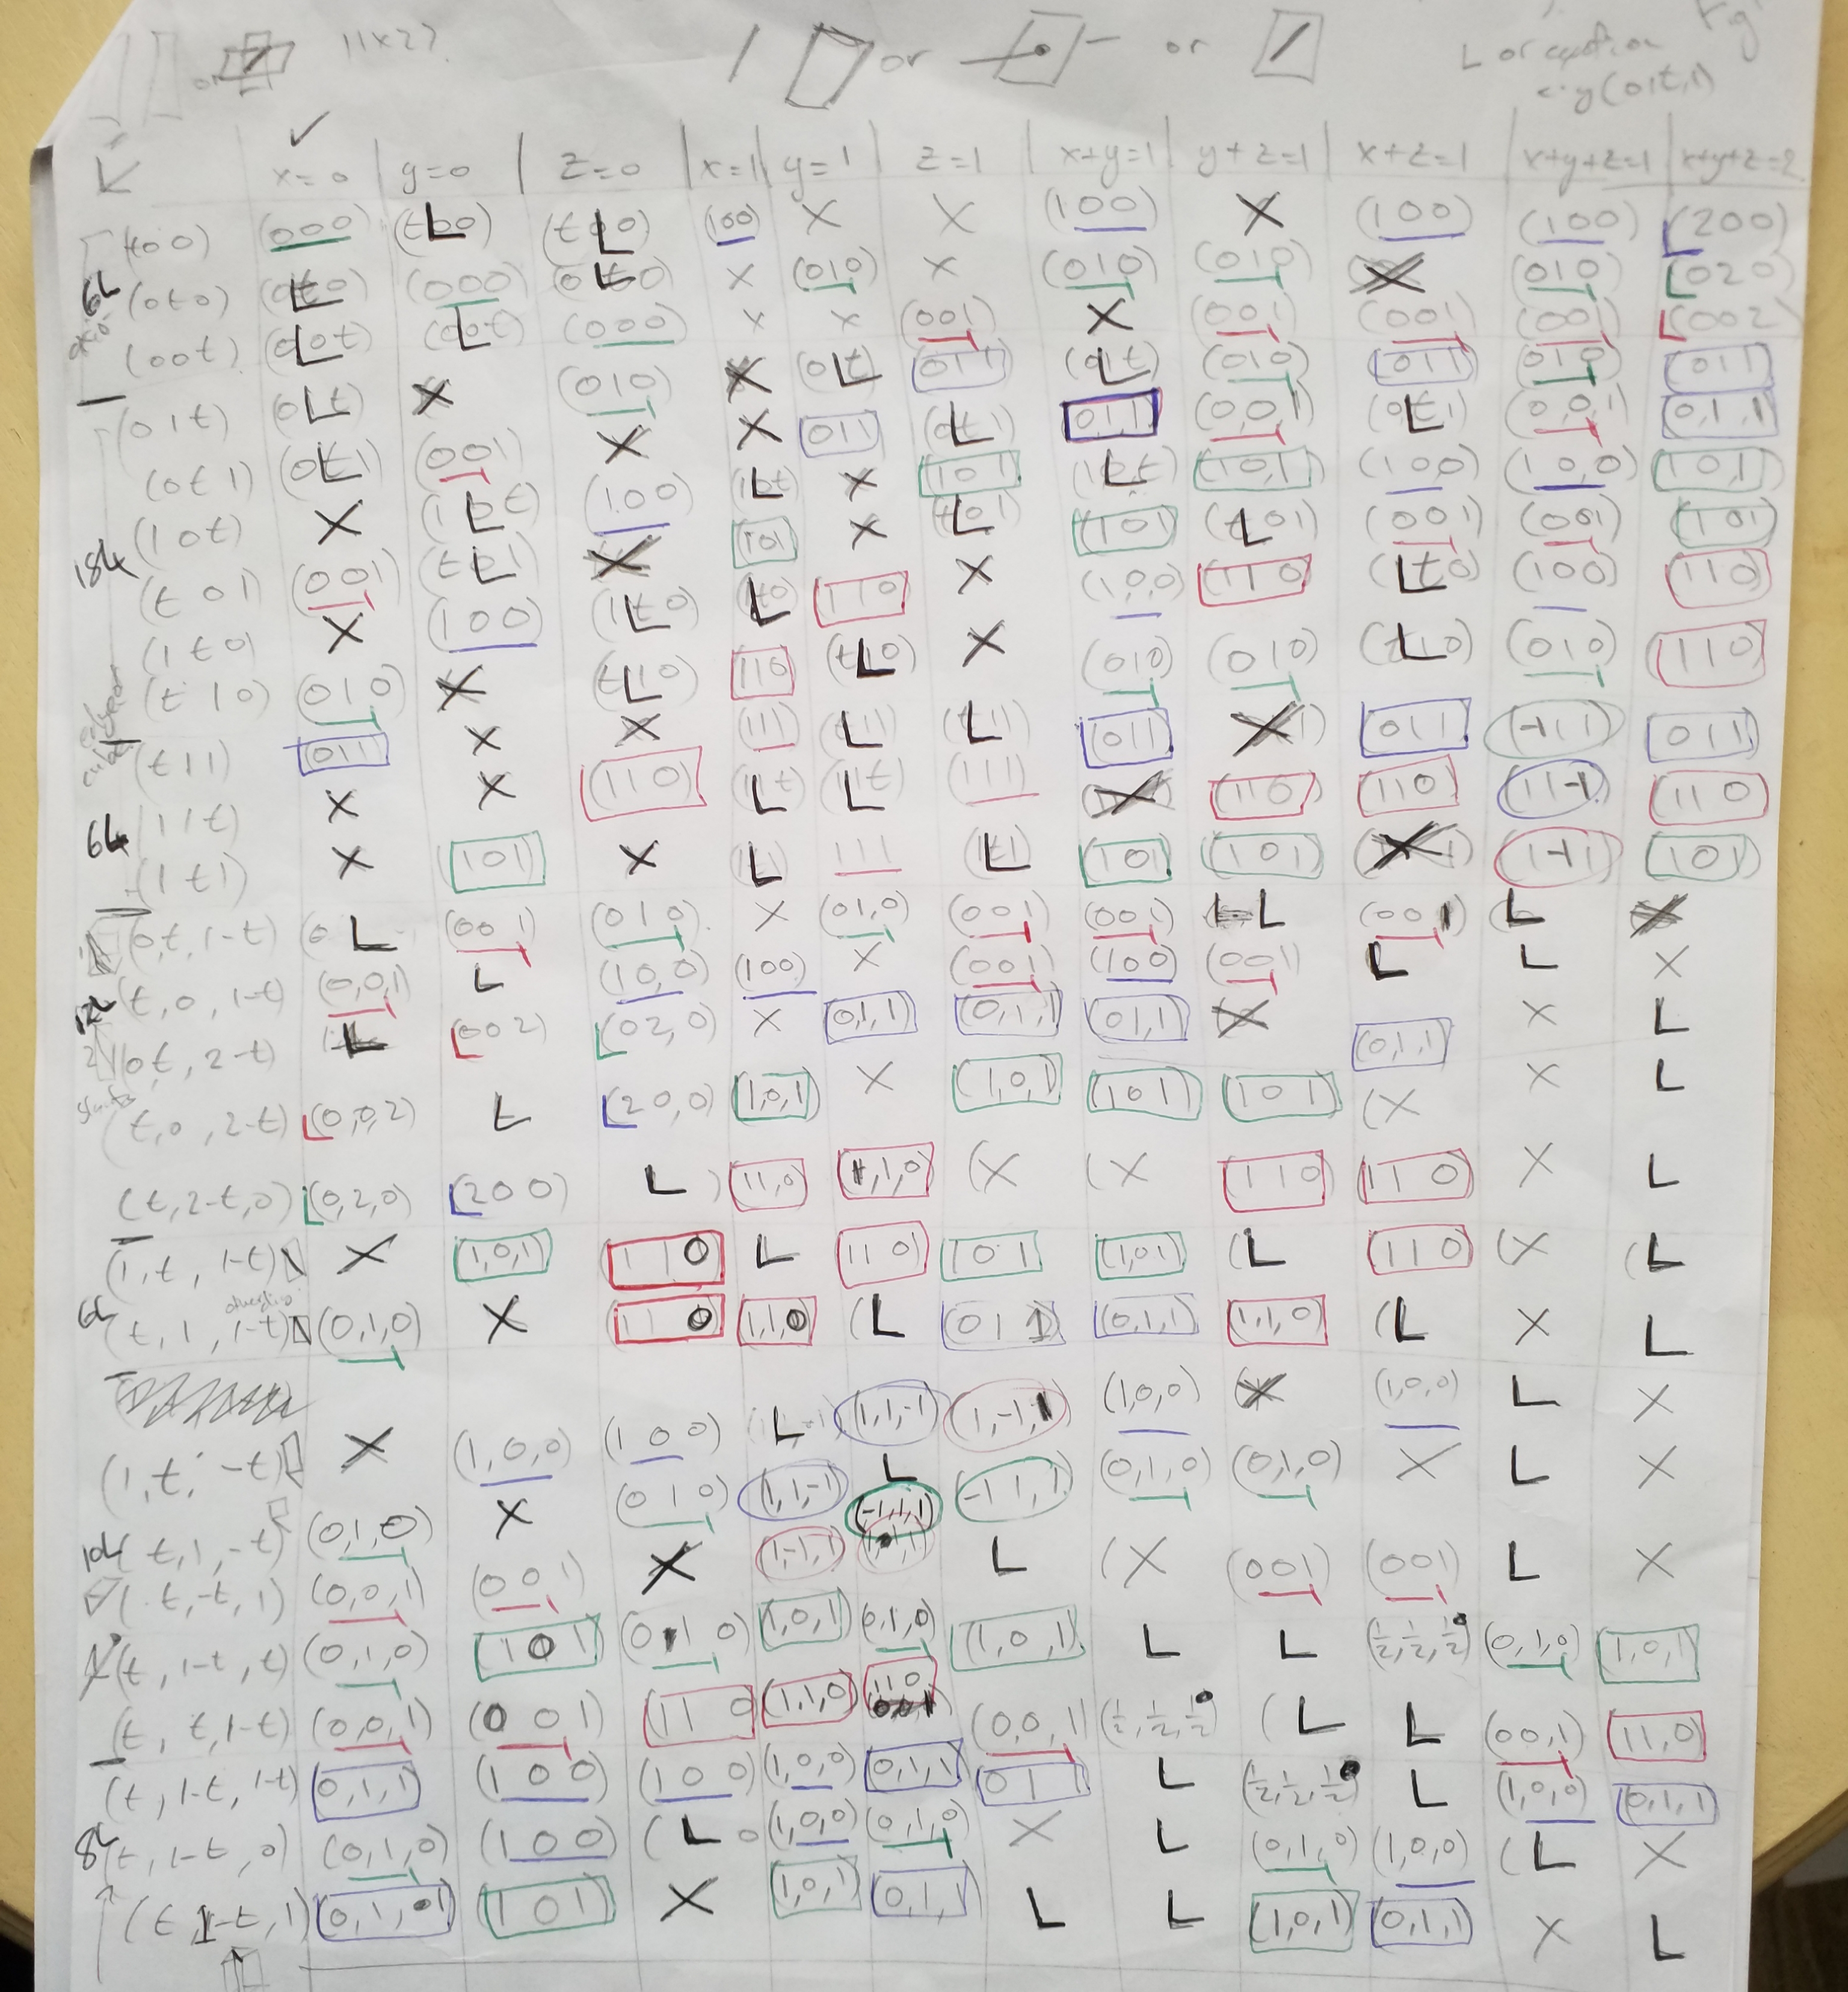
\includegraphics[scale=0.10,angle=0]{29072020 pics/lineplaneint.jpg}  
    \caption{Intersection of lines and planes}
    \label{fig 3}
\end{figure}

We are only interested in the points as the $\mu$ values for lines have already been determined. 

%The number of $L$ are 66.

\begin{remark} Note the points $(2,0,0), (0,2,0), (0,0,2), (-1,1,1),(1,-1,1) ,(1,1,-1)$, these give $6$ bounded tetrahedron regions on the faces of the cube.Once we show the number of bounded region inside the cube is $10$, then we will have $b(\mathcal{A}) \ge 16$, contradicting what we wanted at the start.
\end{remark}


Next we determine the mobius values for the points. For this we need to know which plane each point belongs to and the number of planes. 

\begin{figure}[H]
    \centering
 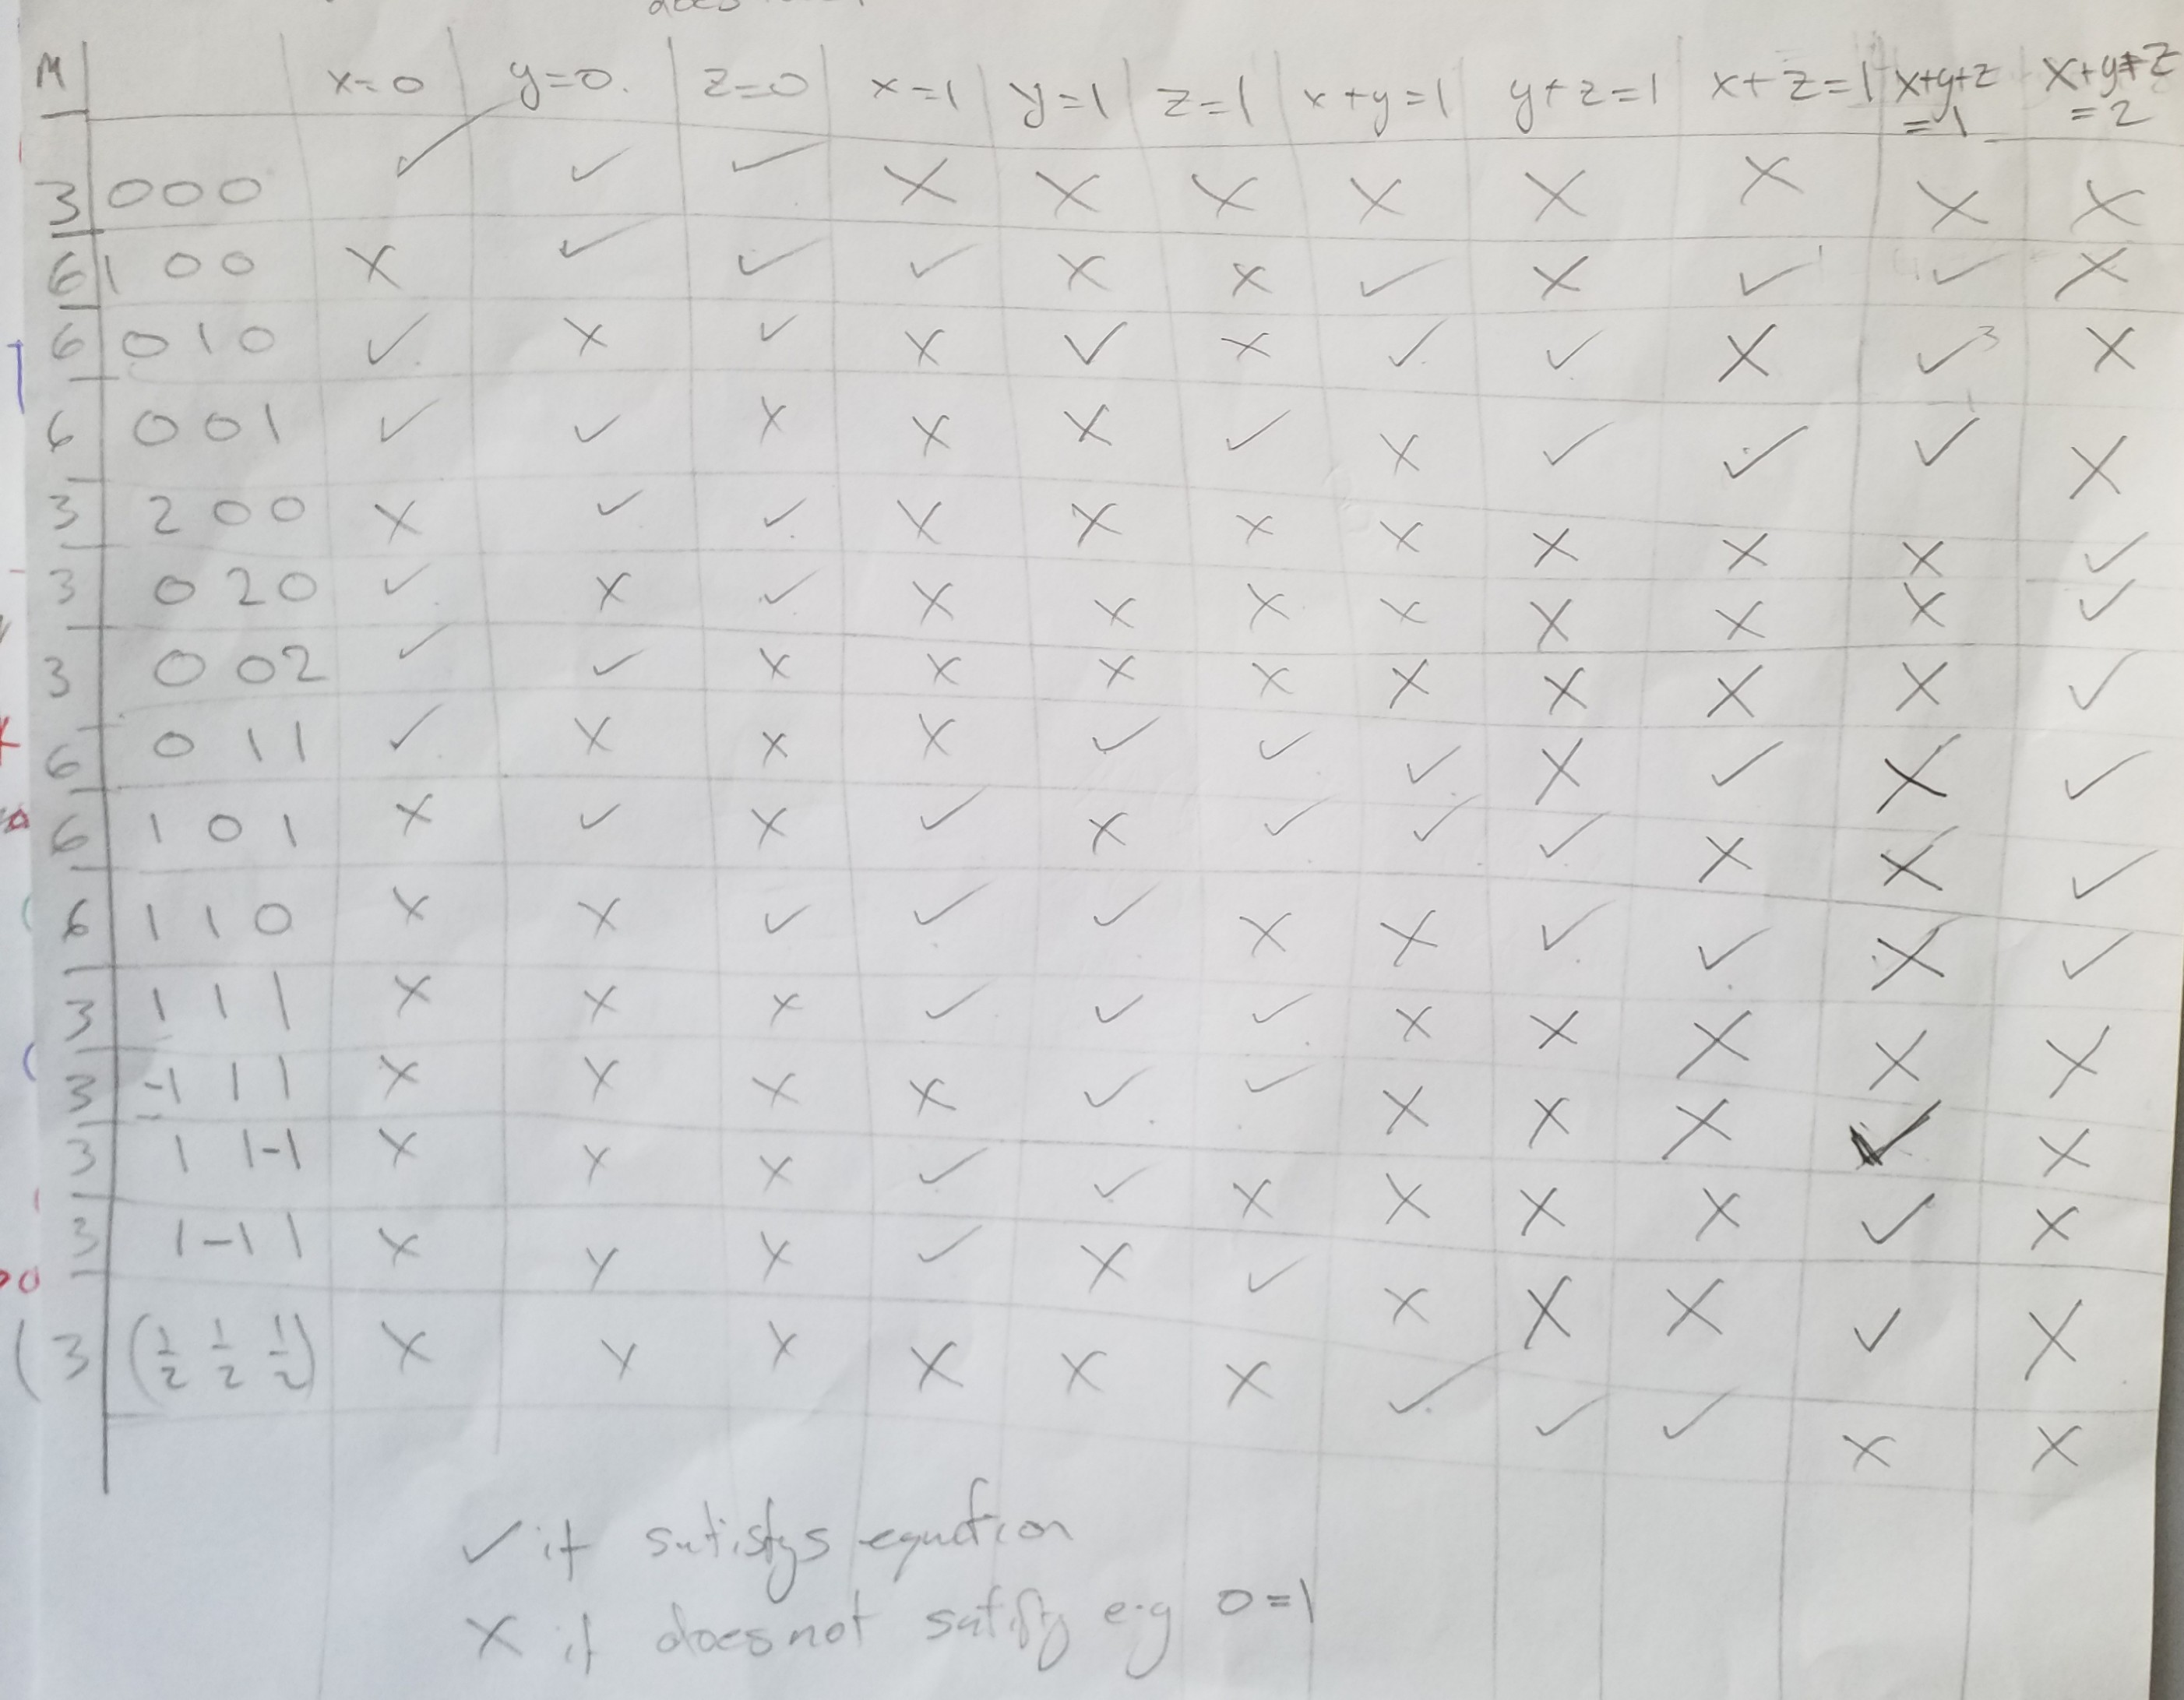
\includegraphics[scale=0.10,angle=0]{29072020 pics/Pointsplane.jpg}  
    \caption{Points in planes}
    \label{pointsplanes}
\end{figure}


 From Figure \ref{fig 3} we can find which planes have the given coordinate. For example the point $(1,1,0)$ is given by $z=0, x=1, y=1, x+y=1,y+z=1, x+z=1, x+y+z=1$ which can be seen in Geoalgebra. We also know from Figure \ref{fig 3} which lines have each point lying in them. From this we can get the Möbius value for the point by noting the number of planes and the sum of mobius values for the lines containing each point. 
 


As all planes have the same Möbius value $-1$. We therefore only need to count the number of planes that give the point (the number of times it appears in different columns in Figure \ref{fig 3}). Note the $\mu$ value for the lines differ so we need to keep track of them. 

\begin{figure}[H]
    \centering
 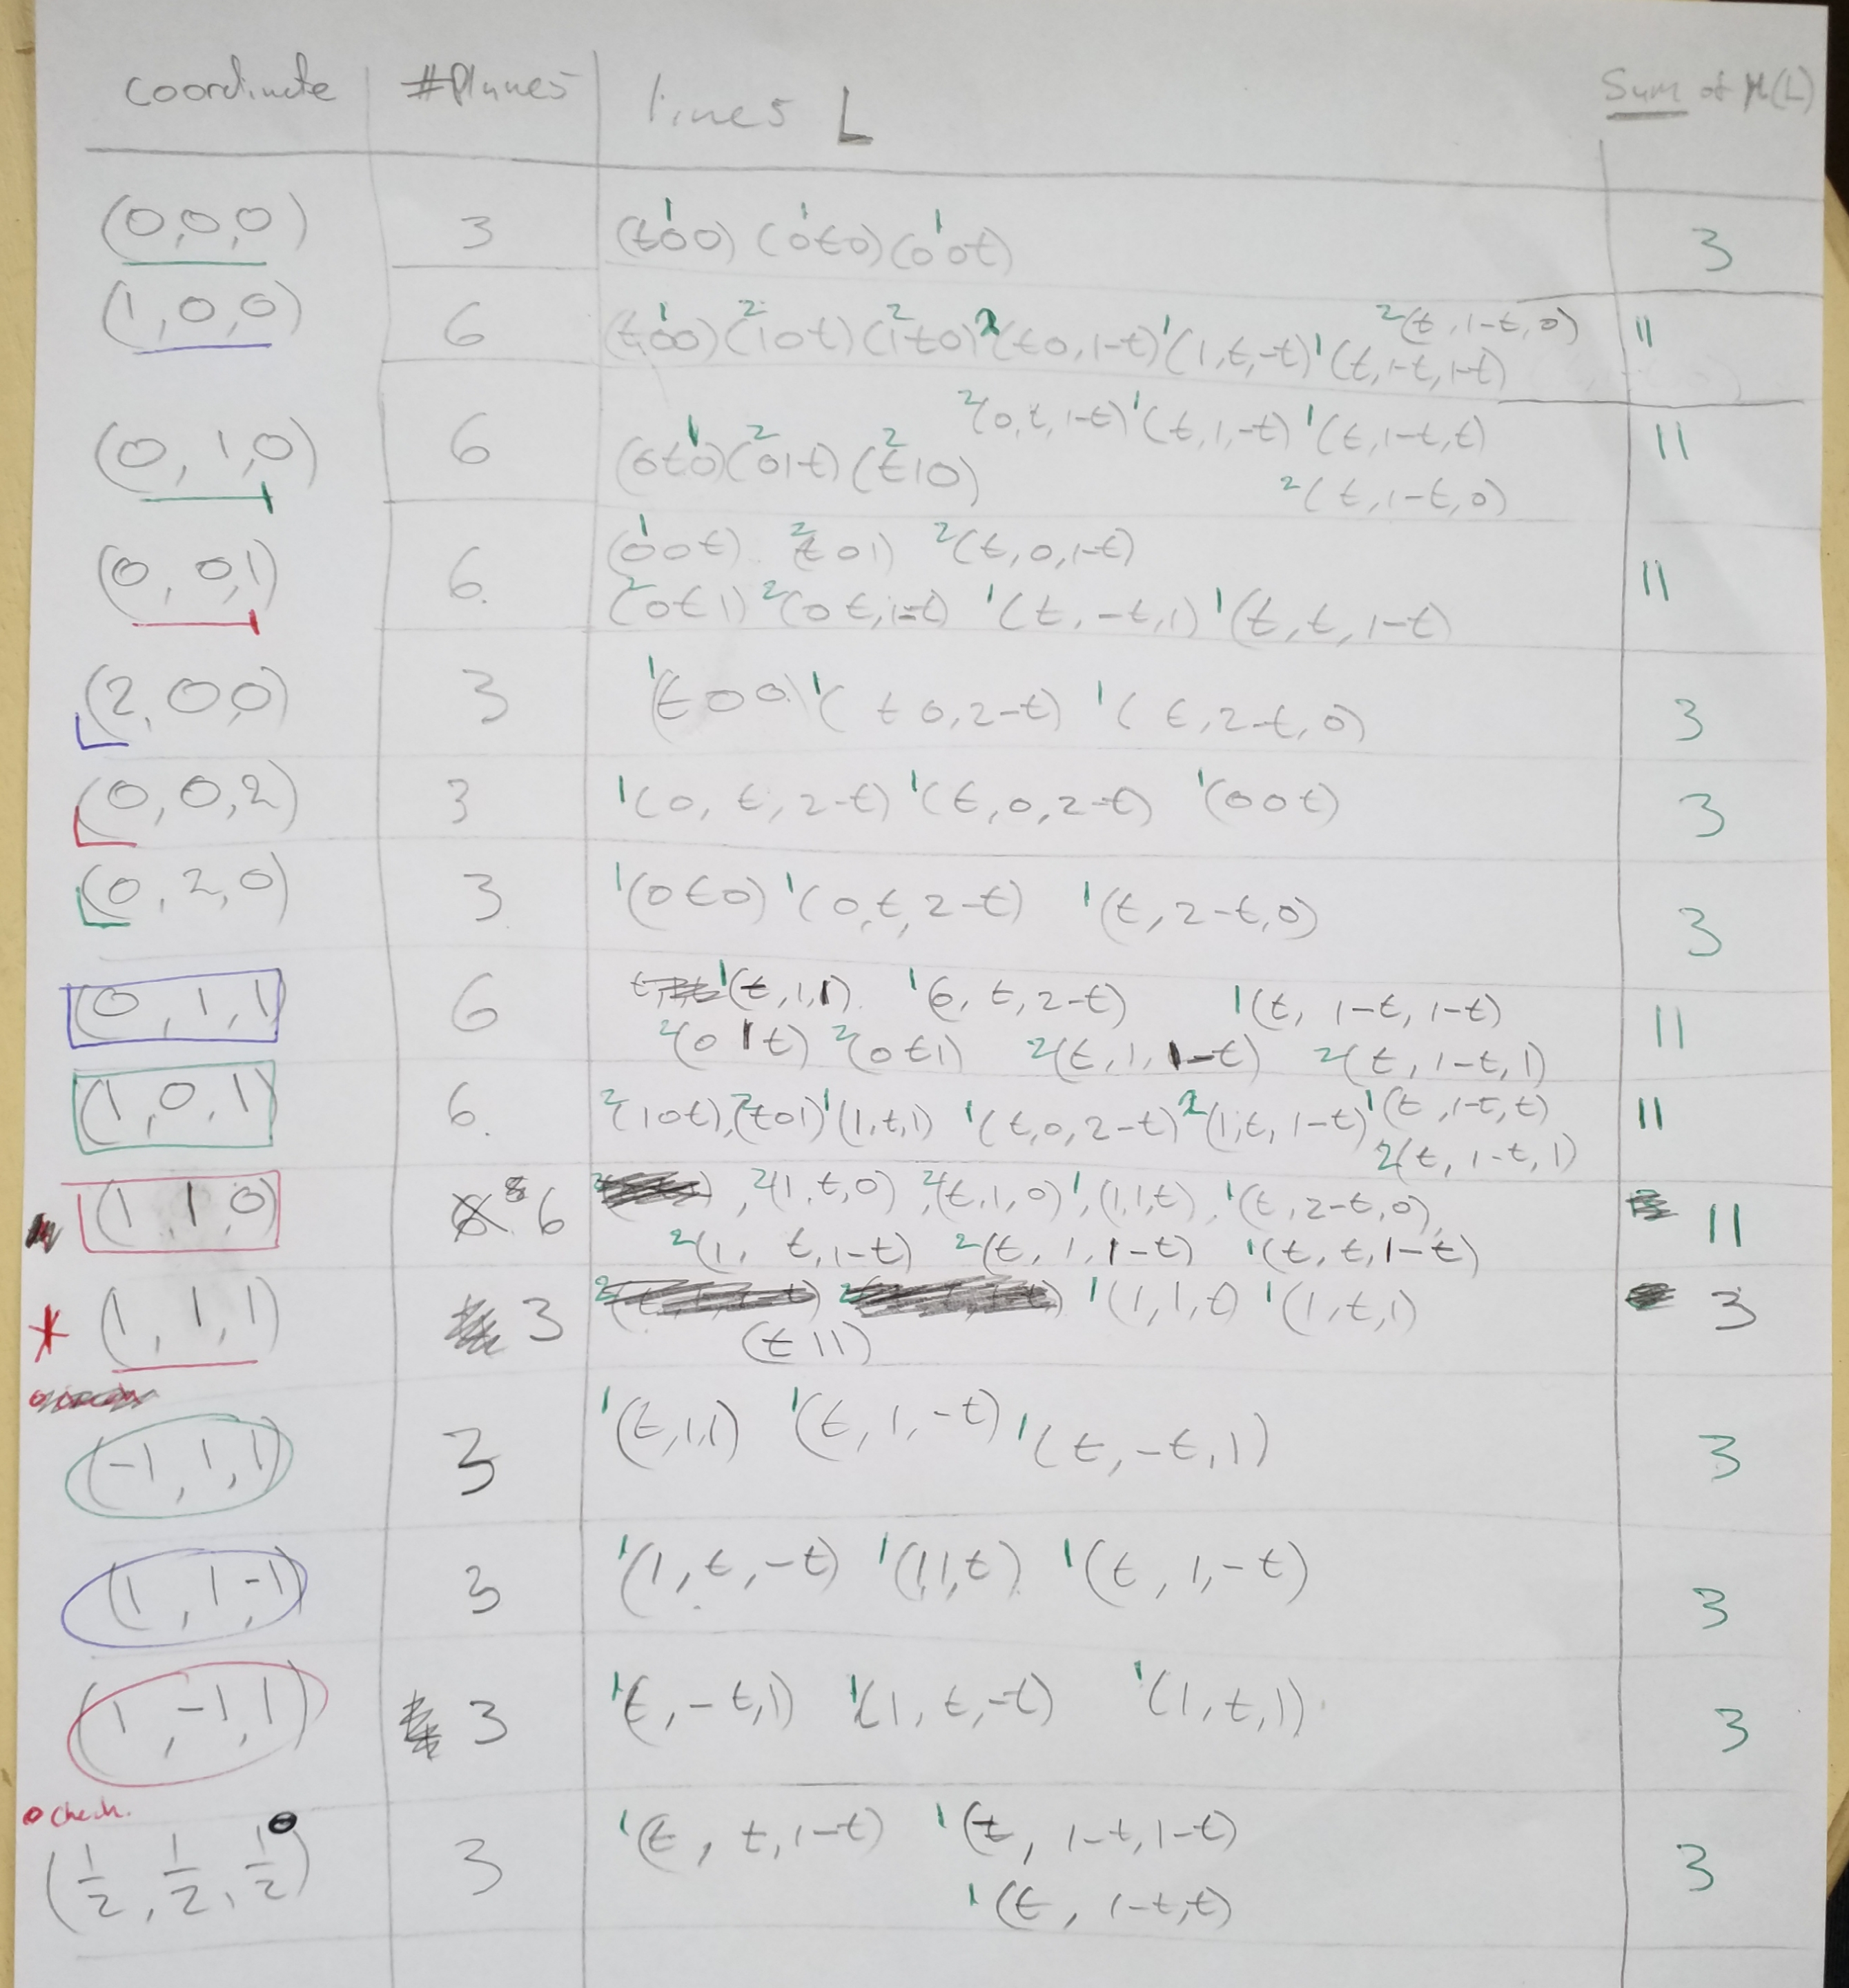
\includegraphics[scale=0.10,angle=0]{29072020 pics/mobpoints.jpg}  
    \caption{Determining the Möbius value of points in poset}
    \label{fig 4}
\end{figure}

For points determined by three planes the Möbius value is $-1$ as, 

$$\mu(\mathbb{R}^3) + \sum_{P\in \mathcal{A}} \mu(P) + \sum_{L \text{given lines}} L + \mu(pt) =0$$
which is,
$$1 -3 + 3 +\mu(pt)=0$$
and so $\mu(pt)=-1$. For points determined by six planes we similarly have,

$$1 -6 +11-\mu(pt)=0,$$

and so $\mu(pt)=-6$. Of the fifteen points we have nine points with $\mu(pt)=-1$ and six points with $\mu(pt)=-6$. Of the $27$ lines we have fifteen of $\mu(L)=1$ and twelve of $\mu(L)=2$. We also have eleven planes in $\mathbb{R}^3$. The characteristic polynomial is therefore,


\begin{align*}
\chi_{\mathcal{A}} (t) &=t^{3} -11t^{2} +(15+12*2)t - (9 * 1 +6*6)\\
&= t^{3} -11t^{2} +39t - 45.
\end{align*}


Applying theorem \ref{Zas} and letting $t=-1$, we have $r(\mathcal{A})=96$. Letting $t=1$, we have $b(\mathcal{A})= 16$. This agrees which the $b(\mathcal{A})$ value we expected. The following diagrams of $\mathcal{A}$ were make using Geoalgebra.

\begin{figure}[H]
    \centering
 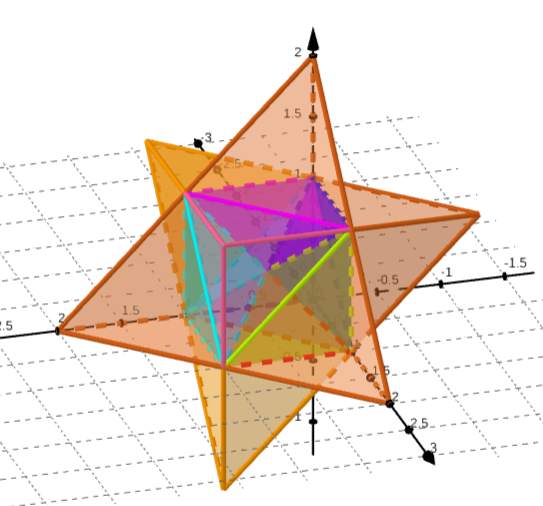
\includegraphics[scale=0.5,angle=0]{29072020 pics/regions1.png}  
    \caption{Bounded regions of $\mathcal{A}$}
    \label{Bounded regions1}
\end{figure}

\begin{figure}[H]
    \centering
 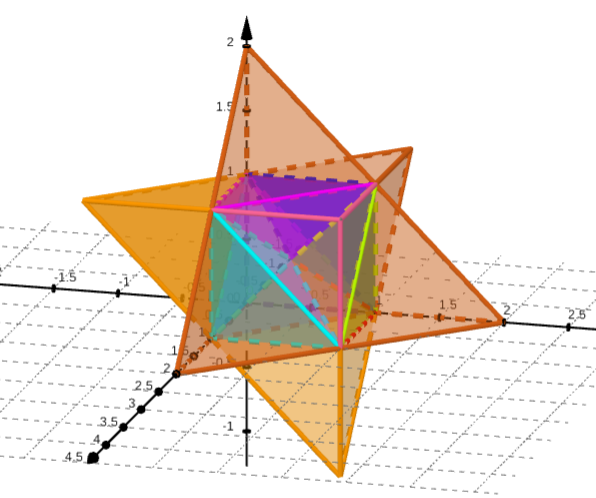
\includegraphics[scale=0.50,angle=0]{29072020 pics/regions2.png}  
    \caption{Bounded regions of $\mathcal{A}$}
    \label{Bounded regions2}
\end{figure}





\end{example}



\printindex

\bibliographystyle{alpha}
\bibliography{bibtex}





\end{document}
